\chapter{多尺度空间建模与混合专家系统的时空交通预测}

\providecommand{\bestres}[1]{\textcolor{red}{\textbf{#1}}}
\providecommand{\secondres}[1]{\textcolor{blue}{\underline{#1}}}

\section{概述}

在上一章中，本文主要面向缺乏显式空间图结构的一般多元时间序列预测问题，从时间多尺度和通道级混合专家的角度缓解时间非平稳与变量分布差异。在此基础上，本章进一步将研究对象扩展至具有显式空间图结构的交通预测问题。交通预测是时空数据挖掘中的经典任务，其目标是根据历史交通传感器观测预测未来若干时刻的交通状态，广泛应用于交通监测、交通管理和路径规划等场景~\cite{tkde-clear,tkde-stman,tkde-stllm,tkde-survey-st,tkde-survey-pretrain,path-rank,mdtp,team,ctvi,msgnet,tkde-poi,tkde-stamh}。与一般多元时间序列预测相比，交通预测中的观测节点与真实路网中的传感器或路段一一对应，节点之间通过道路连接形成显式空间邻接关系。因此，交通预测不仅要建模时间维度的变化，还要同时利用空间拓扑先验刻画节点之间的相互作用。

\begin{figure}[ht]
    \centering
    \fbox{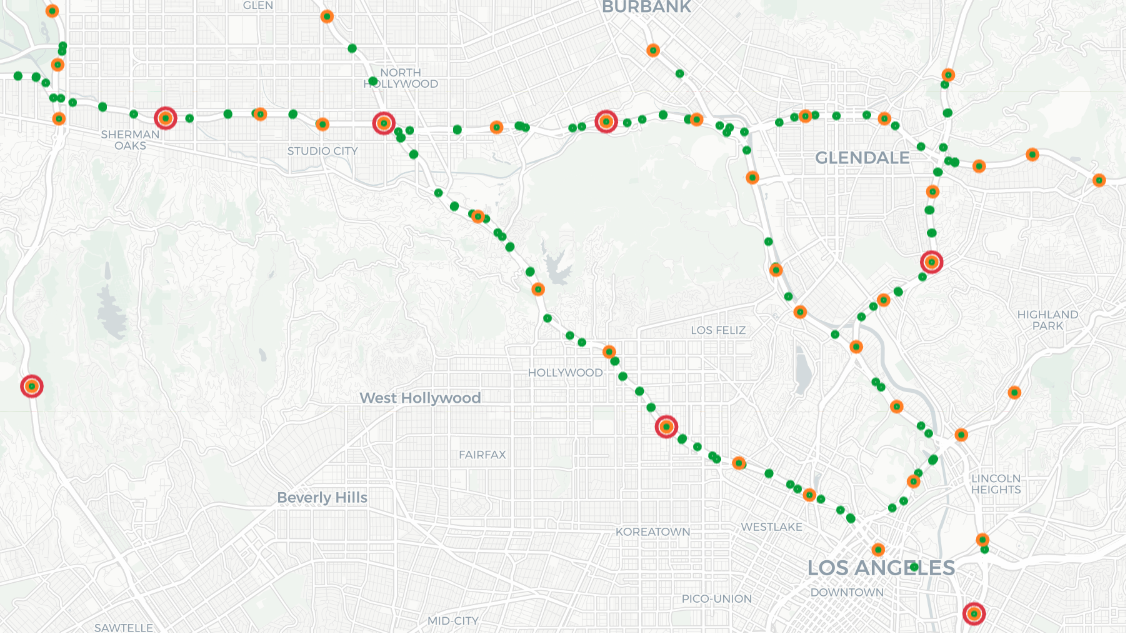
\includegraphics[width=\linewidth]{figure/ch4-metr-realMap.png}}
    \caption{METR-LA 数据集经最远点采样~\cite{fps}后的三个空间尺度的传感器位置}
    \label{fig:ch4_sns_map}
\end{figure}
交通预测的主要挑战来自空间特征和时间特征的提取与融合~\cite{traffic-stf-survey,survey01,tkde-scnn}。现实交通数据通常表现出空间非平稳性，即空间模式会随空间尺度变化而变化~\cite{maup,scale-independent01,mgwr}；同时，交通数据还受到时间非平稳性影响，在不同时段呈现不同的动态模式~\cite{brockwell1991time,revin}。因此，如何有效建模多尺度空间模式，并联合刻画静态与动态时空依赖，是交通预测中尚未充分解决的问题。

\begin{figure}[ht]
    \centering
    \fbox{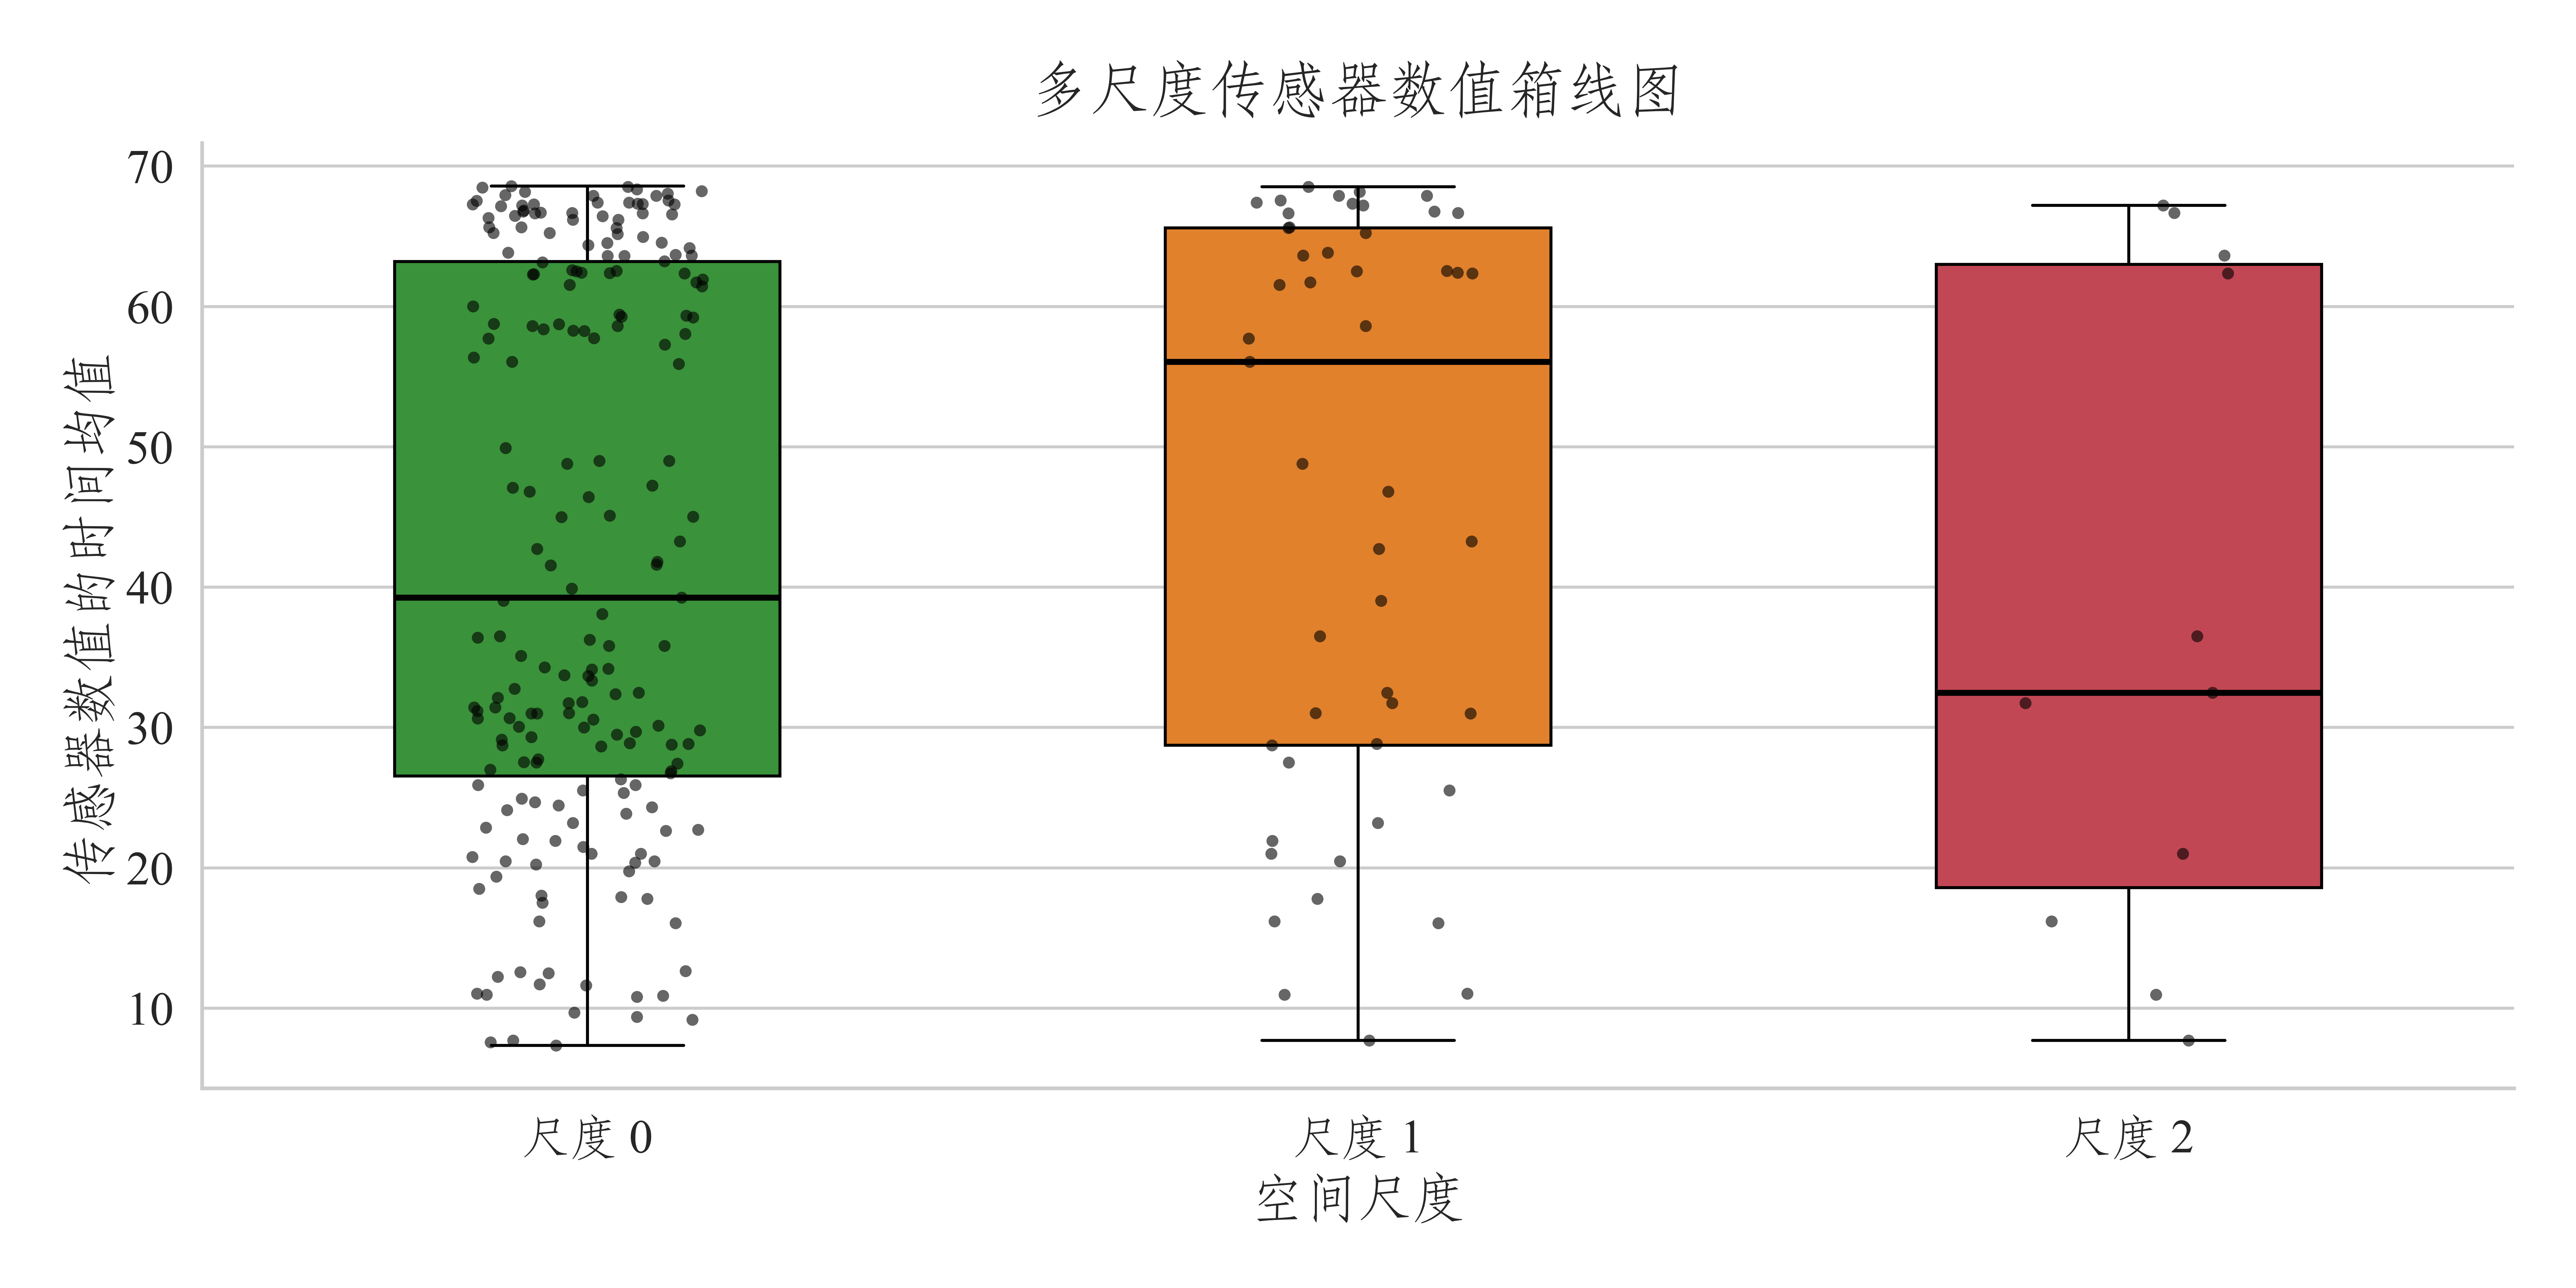
\includegraphics[width=\linewidth]{figure/ch4-metr-scaleDistriDiff.png}}
    \caption{METR-LA 数据集三个空间尺度的传感器数据分布箱线图}
    \label{fig:ch4_sns_dist}
\end{figure}
首先，由空间非平稳性引起的异质空间模式仍未被充分研究。现实交通时空数据中的空间模式具有明显的非均匀性，观测数据分布会随空间尺度变化而发生漂移。为刻画这一问题，本章使用最远点采样算法~\cite{fps} 对 METR-LA 数据集构造三个空间尺度，分别保留 207、51 和 12 个节点。图~\ref{fig:ch4_sns_map} 展示了这三个尺度下的传感器位置，图~\ref{fig:ch4_sns_dist} 展示了各尺度下传感器数据分布的箱线图。可以看到，不同尺度之间的数据分布存在明显差异，说明分别建模不同尺度能够提供互补信息，也进一步说明自适应构造空间尺度并提取尺度特异性特征的必要性。现有研究虽然尝试从多尺度角度建模空间模式，但通常依赖先验知识构造尺度，且大多只考虑原图和一个额外子图两个尺度，难以支持更多尺度或灵活融合~\cite{hgcn,hstgl,stpgnn,gagnn,airformer}。

其次，交通数据中的静态结构和动态时空模式往往同时存在。现有框架通常使用一组共享网络参数对所有时间模式进行统一建模，未显式区分高峰、非高峰等不同时间状态。交通流在一天内通常呈现明显的高峰和非高峰模式，早晚高峰流量较高、夜间流量较低，从而产生时间非平稳性。同时，即使在相同时段内，由道路连接决定的静态局部依赖和跨区域非局部动态依赖也共同决定交通演化。混合专家方法可以将不同时间模式的数据路由到不同专家，从而更灵活地挖掘异质时空依赖。TESTAM 虽然采用全激活混合专家结构分别提取时间、静态图和动态图特征，但其路由发生在所有专家完成计算之后，未实现真正稀疏激活；其硬专家选择策略也限制了静态和动态特征的联合建模。因此，需要一种能够同时建模静态空间结构和动态时间变化，并保持高效稀疏激活的方法。

针对上述问题，本章构建一个融合自适应空间多尺度建模与静动态双混合专家的交通预测框架。该框架通过图池化以数据驱动方式构造多个空间尺度，利用尺度专家和尺度自适应融合提取尺度特异性特征；同时使用稀疏激活的静态图专家和动态图专家分别建模显式拓扑结构与隐式时空依赖，从而在保留路网结构先验的基础上，补充由注意力机制发现的动态跨节点交互。


\section{自适应空间多尺度建模与时空静动态混合专家的交通预测框架}
\label{sec:ch4_method}

\subsection{问题定义与总体框架}
\label{sec:ch4_overall}

沿用第2章记号，将交通路网表示为图 $\mathcal{G}=(\mathcal{V},\mathcal{E},\mathcal{A})$，其中 $\mathcal{V}$ 为节点集合，$N=|\mathcal{V}|$ 为传感器数，$\mathcal{A}\in\mathbb{R}^{N\times N}$ 为邻接矩阵。设历史观测为 $X\in\mathbb{R}^{N\times T}$，其中 $T$ 为历史长度；预测目标为未来 $H$ 个时刻的节点取值 $Y_\mathrm{pred}\in\mathbb{R}^{N\times H}$。模型的目标是学习映射：
\begin{equation}
f_{\theta}:\left(X,\mathcal{G}\right)\mapsto Y_\mathrm{pred}.
\end{equation}

整体框架如图~\ref{fig:ch4_framework} 所示。首先，如第~\ref{sec:ch4_encoder} 节所述，将历史交通数据和时刻信息编码为原始图节点嵌入 $X_{enc}$。随后，该嵌入由两个模块并行处理。空间多尺度混合专家模块见第~\ref{sec:ch4_smsmoe} 节，其首先通过图池化将原始图下采样为多个空间尺度；得到的各尺度子图与原图一起由对应尺度专家处理，每个尺度专家使用图卷积和可学习骨架节点交叉注意力提取尺度特异性特征，并由尺度自适应融合模块进行自适应聚合，得到空间多尺度特征 $X_{SMS}$。静态—动态双混合专家模块见第~\ref{sec:ch4_sdmoe} 节，其通过静态图混合专家和动态图混合专家分别建模静态与动态模式：静态图专家将原始图路由到基于图卷积的专家以捕获显式拓扑结构，动态图专家使用节点级全注意力隐式构造动态图；两类输出拼接为 $X_{SD}$。最后，第~\ref{sec:ch4_fusion} 节所述融合模块将 $X_{SMS}$ 与 $X_{SD}$ 通过门控融合层和 MLP 进一步整合，并由预测层输出未来交通数据。

\begin{figure}[t!]
\centering
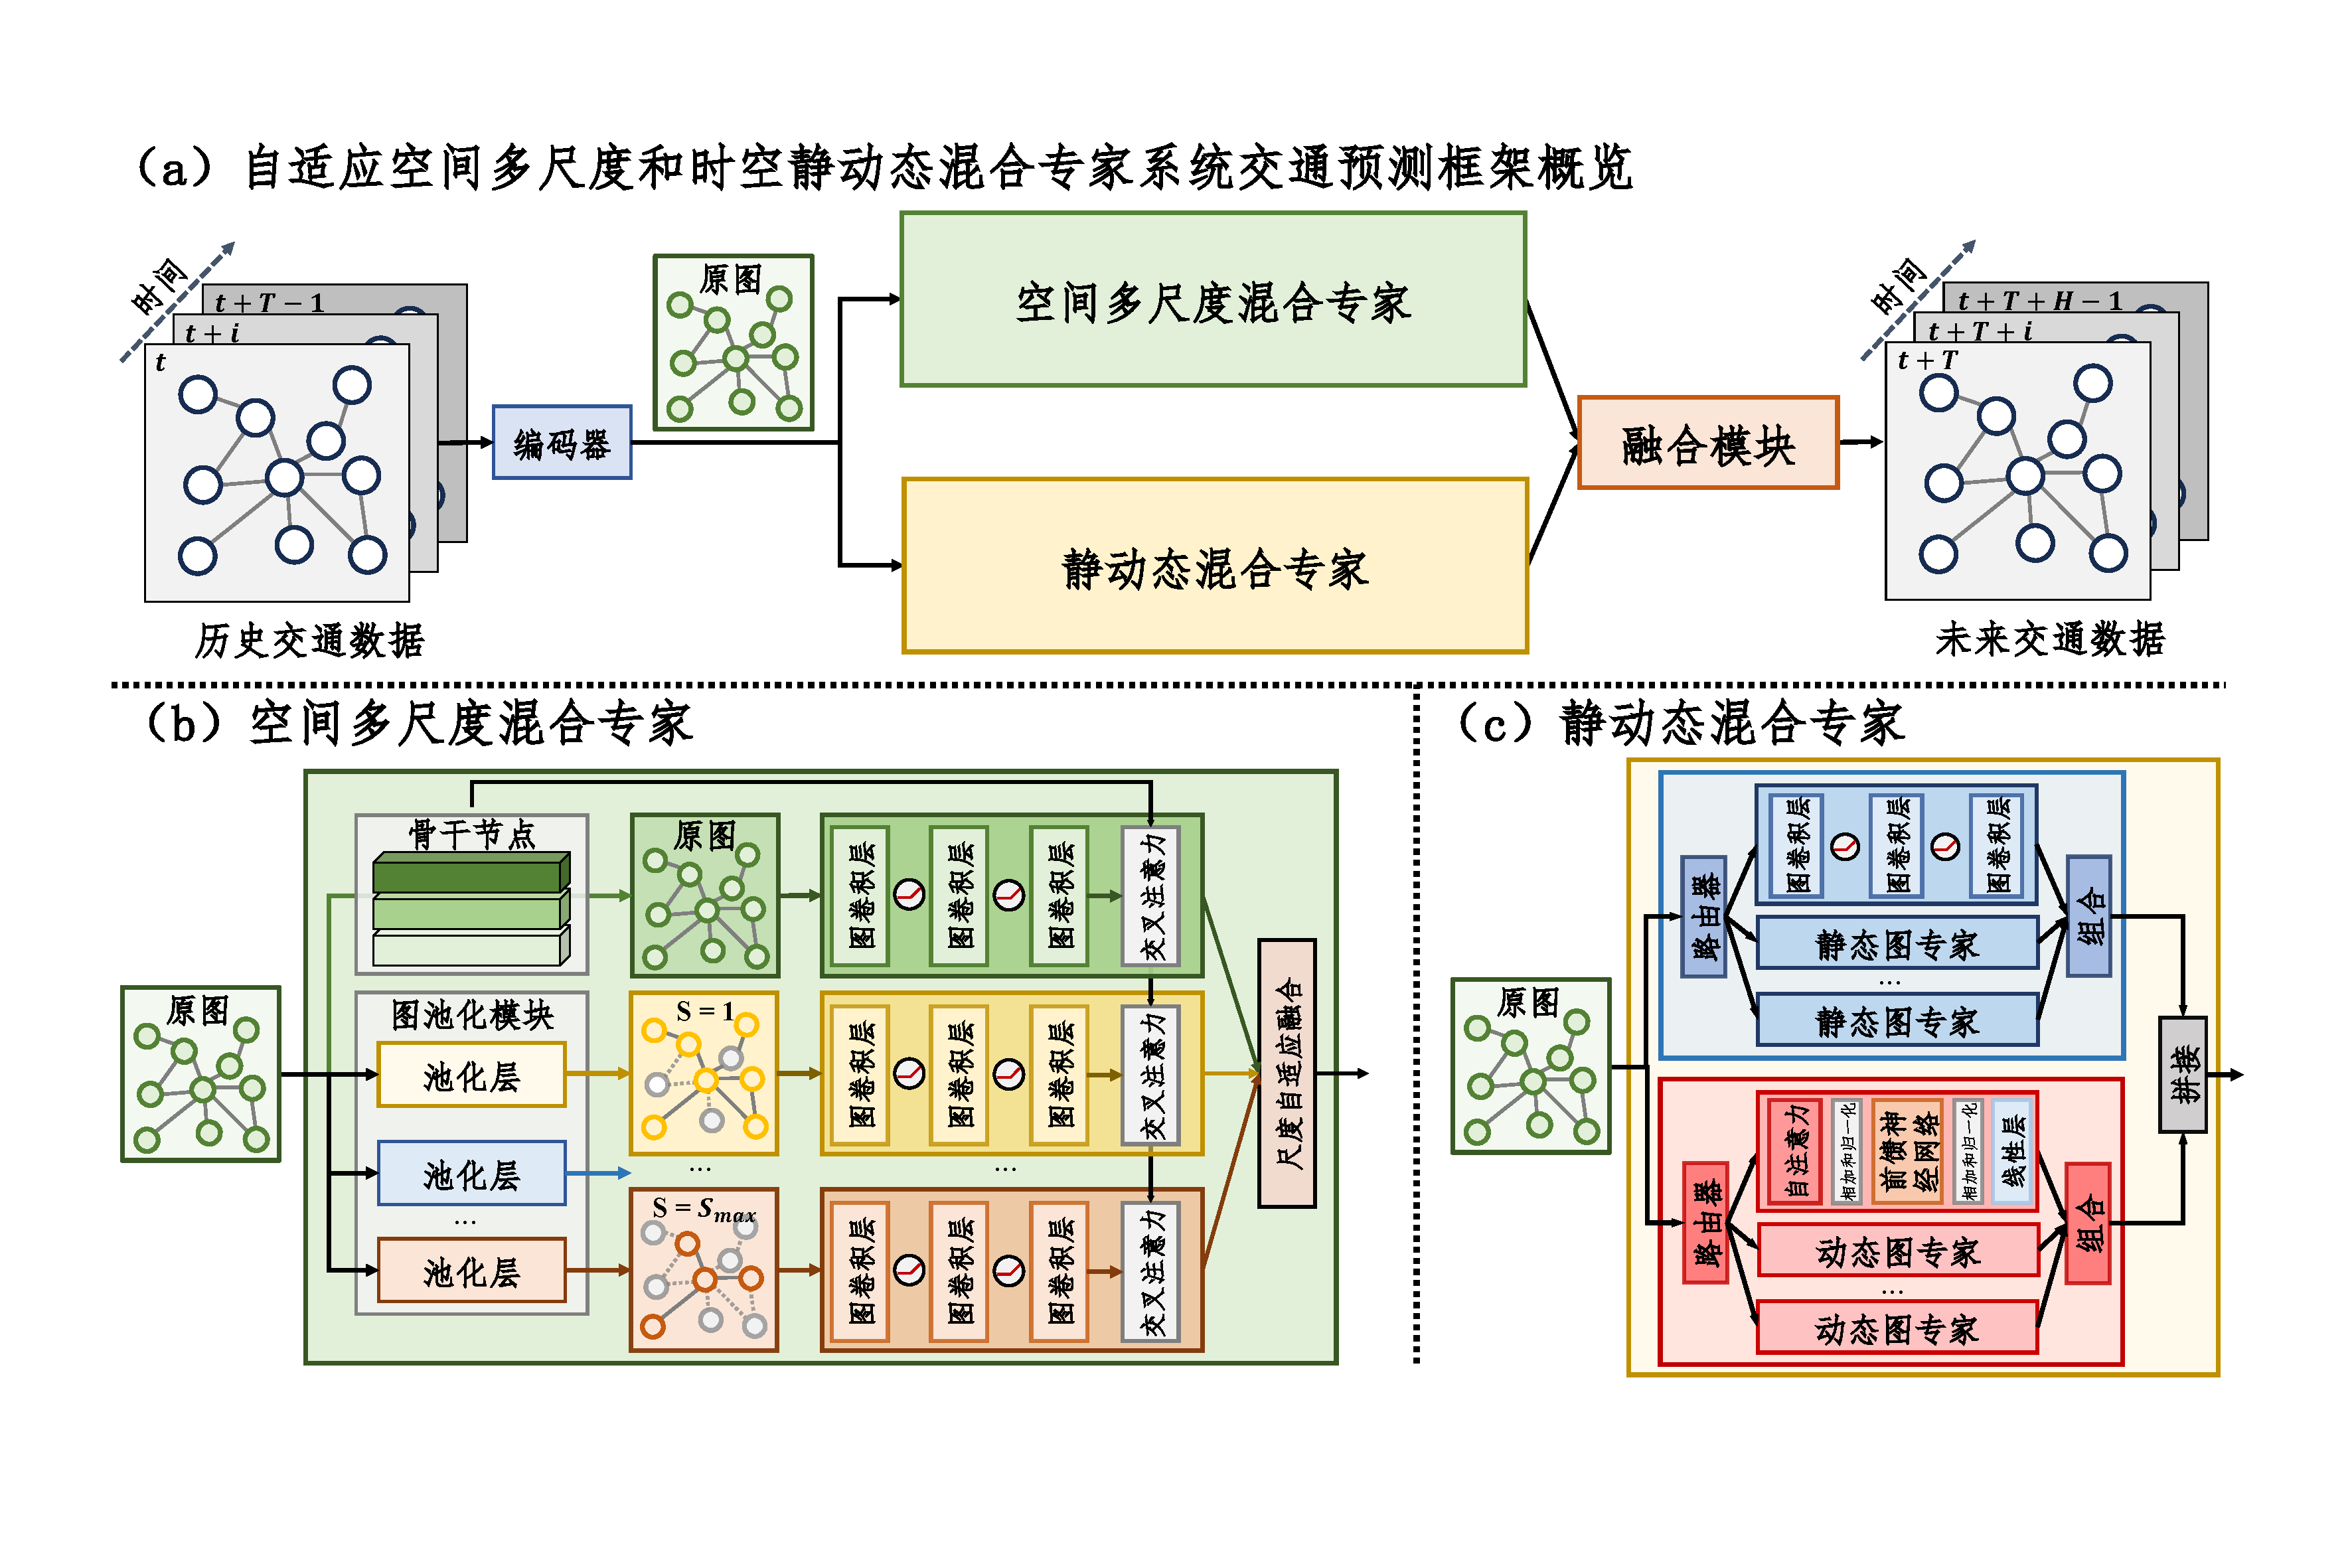
\includegraphics[width=\linewidth]{figure/adams-moe-pipeline.pdf}
\caption{自适应空间多尺度建模与时空静动态混合专家的交通预测框架图}
\label{fig:ch4_framework}
\end{figure}

\subsection{编码器}
\label{sec:ch4_encoder}

为了增强交通数据的表达能力，编码器首先将历史数据编码为原始图节点嵌入。除历史观测 $X\in\mathbb{R}^{N\times T}$ 外，本章还利用日内时间索引和星期索引作为时刻信息。对第 $t$ 个时间步，记日内时间索引和星期索引分别为 $x_{tid,t}$ 和 $x_{diw,t}$，并通过两个可学习嵌入表将其映射为连续向量：
\begin{equation}
e_{tid,t}=\mathrm{Embed}_{tid}\!\left(x_{tid,t}\right),
\end{equation}
\begin{equation}
e_{diw,t}=\mathrm{Embed}_{diw}\!\left(x_{diw,t}\right),
\end{equation}
其中 $e_{tid,t},e_{diw,t}\in\mathbb{R}^{d}$，两个嵌入表的类别数在实现中分别取 $288$ 和 $7$。将第 $n$ 个节点在时刻 $t$ 的观测 $x_{n,t}$ 与两个时刻嵌入拼接，并通过线性层映射到隐空间：
\begin{equation}
x_{enc}^{n,t}=\mathrm{Linear}\!\left(\left[x_{n,t};e_{tid,t};e_{diw,t}\right]\right)\in\mathbb{R}^{d},
\end{equation}
随后沿时间维聚合，时刻嵌入按节点广播，得到编码后的节点嵌入 $X_{enc}\in\mathbb{R}^{N\times d}$，其中 $T$ 为历史时间步数，$N$ 为传感器数，$d$ 为隐层维度。记最后一个时间步的时刻嵌入为 $E_{tid},E_{diw}\in\mathbb{R}^{N\times d}$，$E_{tid},E_{diw}$ 在后续融合模块中作为时刻嵌入再次使用。

\subsection{数据驱动的空间多尺度图构造}
\label{sec:ch4_smsmoe}

为了捕捉交通数据的空间异质性并支持尺度自适应建模，本章提出空间多尺度混合专家模块。该模块由三部分组成：图池化模块反复对原始交通图进行下采样，构造多个空间尺度上的子图；每个尺度对应一个尺度专家，用于提取该尺度下的空间特征；尺度自适应融合模块将这些特征在原始节点空间中合并。其中，融合模块首先通过散布对齐将各尺度特征映射回原始节点，再通过输入自适应尺度门控根据当前输入对各尺度重新加权。整体上，该模块以数据驱动方式发现多尺度空间模式，并在不同尺度之间进行动态融合。

\noindent\textbf{子图构造\ \ } 编码完成后，得到原始图节点嵌入 $X_{enc}^0\in\mathbb{R}^{N\times d}$ 和原始图 $\mathcal{G}_0$。为构造 $S$ 个空间尺度上的子图，使用包含 $S$ 个池化层的图池化模块。对第 $i$ 个池化层，轻量图卷积为原始图 $\mathcal{G}_0$ 中的每个节点生成得分~\cite{sagpool}，并选择得分最高的 $\lfloor N/F^{i}\rfloor$ 个节点构造子图 $\mathcal{G}_i$，其中 $F$ 为尺度缩放因子，$N_i=\lfloor N/F^{i}\rfloor$。为保留结构信息，$\mathcal{G}_i$ 直接从原始图构造，而不是从中间池化图构造：
\begin{equation}
scores_i=\mathrm{GCN}\!\left(X_{enc}^0,\mathcal{A}\right),
\end{equation}
\begin{equation}
\mathrm{idx}_i=\mathrm{TopK}\!\left(scores_i,N_i\right),
\end{equation}
\begin{equation}
X_{enc}^i=\left(\mathcal{A}_{norm}X_{enc}^0\right)_{\mathrm{idx}_i},
\end{equation}
\begin{equation}
\mathcal{A}_i=\mathcal{A}_{\mathrm{idx}_i,\mathrm{idx}_i},
\end{equation}
其中 $X_{enc}^i\in\mathbb{R}^{N_i\times d}$ 为池化后的节点嵌入，$\mathcal{A}_i\in\mathbb{R}^{N_i\times N_i}$ 为子图邻接矩阵，$\mathrm{idx}_i$ 记录保留节点在原始图中的索引。给定 $F$，该过程得到 $S=\lfloor\log_F N\rfloor$ 个子图。图池化流程如算法~\ref{alg:ch4_graph_pooling} 所示。

\begin{algorithm}[t!]
\caption{图池化构造第 $i$ 个尺度子图 $S_i$}
\label{alg:ch4_graph_pooling}
\begin{algorithmic}[1]
\REQUIRE 节点嵌入 $X_{enc}\in\mathbb{R}^{N\times d}$，邻接矩阵 $\mathcal{A}\in\mathbb{R}^{N\times N}$，尺度因子 $F$，池化层索引 $i$
\ENSURE 池化节点嵌入 $X_{enc}^i\in\mathbb{R}^{N_i\times d}$，池化邻接矩阵 $\mathcal{A}_i\in\mathbb{R}^{N_i\times N_i}$，保留节点索引 $\mathrm{idx}_i$
\STATE $N_i\leftarrow\lfloor N/F^{i}\rfloor$
\STATE 构造单位矩阵 $\mathcal{I}\in\mathbb{R}^{N\times N}$
\STATE $\tilde{\mathcal{A}}\leftarrow\mathcal{A}+\mathcal{I}$
\STATE $\mathcal{D}\leftarrow\mathrm{diag}\!\left(\sum_j\tilde{\mathcal{A}}_{ij}\right)$
\STATE $\mathcal{A}_{norm}\leftarrow\mathcal{D}^{-1/2}\tilde{\mathcal{A}}\mathcal{D}^{-1/2}$
\STATE $X_{agg}\leftarrow\mathcal{A}_{norm}X_{enc}$
\STATE $H\leftarrow\mathrm{ReLU}\!\left(W_1X_{agg}\right)$
\STATE $scores_i\leftarrow W_2H\in\mathbb{R}^{N}$
\STATE $\mathrm{idx}_i\leftarrow\mathrm{TopK}\!\left(scores_i,N_i\right)$
\STATE $\hat{X}_{enc}^i\leftarrow X_{enc}[\mathrm{idx}_i]\odot\sigma\!\left(scores_i[\mathrm{idx}_i]\right)$
\STATE $X_{enc}^i\leftarrow\hat{X}_{enc}^i+\left(\mathcal{A}_{norm}X_{enc}\right)[\mathrm{idx}_i]$
\STATE $\mathcal{A}_i\leftarrow\mathcal{A}[\mathrm{idx}_i,\mathrm{idx}_i]$
\STATE \RETURN $X_{enc}^i,\mathcal{A}_i,\mathrm{idx}_i$
\end{algorithmic}
\end{algorithm}

\noindent\textbf{尺度特异性特征提取\ \ } 通过在不同尺度上应用图池化模块，得到层次图集合 $G=\{\mathcal{G}_0,\mathcal{G}_1,\ldots,\mathcal{G}_S\}$ 以及对应节点嵌入 $\mathcal{X}=\{X_{enc}^0,\ldots,X_{enc}^{(S)}\}$。为提取跨尺度空间模式，为每个尺度设计基于图卷积的尺度专家。对第 $i$ 个尺度图，堆叠 $L$ 层图卷积。第 $l$ 层计算为
\begin{equation}
    \hat{\mathcal{A}_i}=\left(D_i\right)^{-\frac12}\mathcal{A}_i\left(D_i\right)^{-\frac12},
\end{equation}
\begin{equation}
    Z_i^0=\hat{\mathcal{A}_i}X_{enc}^iW^0_i+b^0_i,
\end{equation}
\begin{equation}
    Z_i^l=\mathrm{ReLU}\!\left(\hat{\mathcal{A}_i}Z_i^{l-1}W^l_i+b^l_i\right),
\end{equation}
其中 $\hat{\mathcal{A}_i}$ 为归一化邻接矩阵，$D_i$ 为度矩阵，$W^l_i,b^l_i$ 为可学习参数。

为了向尺度表示引入不依赖输入且空间上更稳定的结构特征，空间多尺度混合专家模块设置可学习骨干节点 $E_{sk}\in\mathbb{R}^{N_{\mathrm{sk}}\times d_{\mathrm{sk}}}$。骨干节点作为全局键和值嵌入，在每个尺度上与图卷积后的特征进行交叉注意力：
\begin{equation}
    Q_i=Z_i^{L-1}W^{(i,Q)},
\end{equation}
\begin{equation}
    E_{sk}^i=\mathrm{Softmax}\!\left(\frac{1}{\sqrt{d_{\mathrm{sk}}}}Q_iE_{sk}^{\top}\right)E_{sk},
\end{equation}
其中 $E_{sk}^i\in\mathbb{R}^{N_i\times d_{\mathrm{sk}}}$ 为输入无关的结构特征，$Z_i^{L-1}$ 为图卷积最后一层前的隐状态，$Z_i^L$ 为图卷积输出。将 $E_{sk}^i$ 与 $Z_i^L$ 拼接，得到尺度特征 $X_s^i\in\mathbb{R}^{N_i\times d_m}$，其中 $d_m=d_o+d_{\mathrm{sk}}$。所有尺度专家完成后，得到多尺度空间特征集合 $\mathcal{X}_s=\{X_s^i\mid i=0,\ldots,S\}$。

\noindent\textbf{尺度自适应融合\ \ }
不同尺度图包含不同数量的节点，因此尺度特征不能直接相加。与沿节点维度重新扩展池化表示不同，尺度自适应融合模块利用池化索引 $\mathrm{idx}_i$ 所编码的物理对应关系，在原始节点空间中融合多尺度特征。该模块首先通过无参数的散布对齐将所有尺度特征映射回原始节点集合，再通过输入自适应尺度门控确定各尺度对当前输入的贡献。

\textbf{散布对齐。} 对第 $i$ 个尺度特征 $X_s^i\in\mathbb{R}^{N_i\times d_m}$，根据 $\mathrm{idx}_i$ 将其散布回原始 $N$ 个节点：
\begin{equation}
\tilde{X}_s^i[n]=\sum_{k:\mathrm{idx}_i[k]=n}X_s^i[k],
\qquad n=1,\ldots,N,
\end{equation}
最细尺度保持不变，即 $\tilde{X}_s^0=X_s^0$。由于 $\mathrm{idx}_i$ 包含互不相同的索引，每个池化节点被恢复到其在交通网络中的原始位置，其余 $N-N_i$ 个节点置为零向量。

\textbf{输入自适应尺度门控。} 为实现自适应多尺度空间融合，使用依赖输入的门控机制控制不同尺度特征的组合。首先对所有节点取平均，得到当前样本的上下文向量：
\begin{equation}
c=\frac{1}{N}\sum_{n=1}^{N}X_{enc}^0[n]\in\mathbb{R}^{d},
\end{equation}
然后使用轻量门控网络和 Softmax 生成各尺度权重：
\begin{equation}
g=\mathrm{Softmax}\!\left(W_2\mathrm{ReLU}\!\left(W_1c+b_1\right)+b_2\right),
\end{equation}
其中 $g\in\mathbb{R}^{S+1}$ 且 $\sum_{i=0}^{S}g_i=1$。这样，每个尺度的贡献取决于当前交通条件：模型可以增强对当前输入最有信息量的尺度，同时抑制其他尺度。

\textbf{自顶向下尺度混合。} 最细尺度特征来自原始图，最粗尺度特征来自节点最少的子图。由于粗尺度捕捉更宏观的模式，本章采用自顶向下混合策略~\cite{timemixer}：
\begin{equation}
    h^S=\tilde{X}_s^S,
\end{equation}
\begin{equation}
    h^i=W_ih^{i+1}+\tilde{X}_s^i,
\qquad i=S-1,\ldots,0,
\end{equation}
其中 $W_i\in\mathbb{R}^{d_m\times d_m}$ 为可学习参数。通过该递归路径，粗尺度的宏观信息被逐步投影并注入细尺度。最后，将门控尺度特征与自顶向下混合特征相加并投影回编码器隐空间：
\begin{equation}
X_{SMS}=W_O\left(\sum_{i=0}^{S}g_i\tilde{X}_s^i+h^0\right)\in\mathbb{R}^{N\times d},
\end{equation}
其中 $W_O\in\mathbb{R}^{d\times d_m}$ 为可学习参数。尺度自适应融合流程如算法~\ref{alg:ch4_scale_fusion} 所示。

\begin{algorithm}[t!]
\caption{带散布对齐的尺度自适应融合}
\label{alg:ch4_scale_fusion}
\begin{algorithmic}[1]
\REQUIRE 多尺度特征 $\mathcal{X}_s=\{X_s^i\mid i=0,\ldots,S\}$，池化索引 $\{\mathrm{idx}_i\mid i=1,\ldots,S\}$，编码输入 $X_{enc}^0$
\ENSURE 空间多尺度特征 $X_{SMS}\in\mathbb{R}^{N\times d}$
\STATE $\tilde{X}_s^0\leftarrow X_s^0$
\FOR{$i=1$ to $S$}
    \STATE $\tilde{X}_s^i\leftarrow\mathbf{0}\in\mathbb{R}^{N\times d_m}$
    \STATE $\tilde{X}_s^i[\mathrm{idx}_i]\leftarrow X_s^i$
\ENDFOR
\STATE $c\leftarrow\frac{1}{N}\sum_{n=1}^{N}X_{enc}^0[n]$
\STATE $g\leftarrow\mathrm{Softmax}\!\left(W_2\mathrm{ReLU}\!\left(W_1c+b_1\right)+b_2\right)$
\STATE $h\leftarrow\tilde{X}_s^S$
\FOR{$i=S-1$ to $0$}
    \STATE $h\leftarrow W_ih+\tilde{X}_s^i$
\ENDFOR
\STATE $X_{SMS}\leftarrow W_O\left(\sum_{i=0}^{S}g_i\tilde{X}_s^i+h\right)$
\STATE \RETURN $X_{SMS}$
\end{algorithmic}
\end{algorithm}

\subsection{静态—动态双混合专家模块}
\label{sec:ch4_sdmoe}

为联合建模静态空间结构和动态时间变化，本章设计静态—动态双混合专家模块，包含两个轻量、稀疏激活的混合专家。静态图混合专家使用路由器将交通数据分配到不同的静态图专家，基于图卷积的专家用于捕捉静态图中的显式拓扑结构；动态图混合专家则并行地使用节点级全注意力动态图专家，挖掘动态图中的隐式时间依赖。两类组件共同实现静态和动态时空特征的统一建模。

\noindent\textbf{静态图混合专家\ \ } 为根据时空特征将数据路由到不同专家，定义可学习节点嵌入 $E_n\in\mathbb{R}^{N\times d}$，并将其与 $X_{enc}$ 拼接，得到路由输入 $X_{sg}$。该设计注入静态空间信息以辅助专家选择。门控以整段时间内整张图的时空特征为输入，聚合出每个专家的路由得分，并在批量维度上对每个样本分别进行 Top-$k$ 选择。路由器使用全连接层实现：
\begin{equation}
    X_g=W_g^l\left(\mathrm{ReLU}\!\left(X_{sg}W_g^0\right)W_g^1\right),
\end{equation}
\begin{equation}
    X_n=W_n^l\left(\mathrm{ReLU}\!\left(X_{sg}W_n^0\right)W_n^1\right),
\end{equation}
其中 $W_g^l,W_n^l\in\mathbb{R}^{N_e\times N}$，$W_g^0,W_n^0\in\mathbb{R}^{2E\times h}$，$W_g^1,W_n^1\in\mathbb{R}^{h\times 1}$，$h$ 为隐层维度，$N_e$ 为专家数。随后使用噪声门控技术~\cite{moe} 选择 Top-$k$ 个专家并计算权重：
\begin{equation}
G\!\left(X_{enc}\right)=\mathrm{Softmax}\!\left(\mathrm{KeepTopK}\!\left(H\!\left(X_{enc}\right),k\right)\right),
\end{equation}
\begin{equation}
H\!\left(X_{enc}\right)=W_e\left(X_g+\gamma\cdot\mathrm{Softplus}\!\left(X_n\right)\right),
\end{equation}
\begin{equation}
\mathrm{KeepTopK}(v,k)_i=
\left\{
\begin{array}{ll}
v_i, & v_i \ \mbox{为}\ v \ \mbox{的前}\ k\ \mbox{个最大元素},\\
-\infty, & \mbox{否则}.
\end{array}
\right.
\end{equation}
其中 $\gamma\sim\mathcal{N}(0,1)$。噪声项用于重采样并稳定噪声门控，Softplus 保持门控信号为正。路由完成后，$X_{enc}$ 被送入选中的 $k$ 个静态图专家，每个专家堆叠 $N_s$ 层图卷积：
\begin{equation}
    X_{se}^1=\mathrm{GCNLayer}_0\!\left(X_{enc},\hat{\mathcal{A}}\right),
\end{equation}
\begin{equation}
    X_{se}^{i+1}=\mathrm{GCNLayer}_i\!\left(X_{\mathrm{se}}^{(i)},\hat{\mathcal{A}}\right).
\end{equation}
被选中专家的输出按门控权重聚合：
\begin{equation}
X_{SG}=\sum_{j=1}^{k}G_j\!\left(X_{enc}\right)X_{se,j}^{N_s},
\end{equation}
其中 $X_{SG}\in\mathbb{R}^{N\times d_S}$ 为静态图特征，$d_S$ 为输出维度。

\noindent\textbf{动态图混合专家\ \ } 动态图混合专家采用与静态图混合专家相同的稀疏激活结构，但其路由信号仅由 $X_{enc}$ 计算，使路由器能够自适应区分隐式时间模式，而不依赖预先给定的空间结构。被选中的动态图专家使用节点级全自注意力提取动态时空特征：
\begin{equation}
    X_{att}=\mathrm{Softmax}\!\left(\frac{\left(X_{enc}W^{Q}\right)\left(X_{enc}W^{K}\right)^{\top}}{\sqrt{d}}\right)X_{enc}W^{V},
\end{equation}
\begin{equation}
    X_{de}=\mathrm{FFN}\!\left(X_{att}\right),
\end{equation}
其中 $W^{Q},W^{K},W^{V}$ 为可学习投影矩阵，$d$ 为投影维度，注意力在节点维上计算。
通过注意力矩阵，该机制隐式诱导动态图，并建模超出局部邻域的跨节点交互。与受静态图拓扑约束的静态图专家不同，动态图专家能够捕捉随时间演化且不局限于局部邻近关系的依赖。专家输出经门控权重聚合，得到动态图特征 $X_{DG}\in\mathbb{R}^{N\times d_D}$。最后，将静态图和动态图特征拼接：
\begin{equation}
X_{SD}=\left[X_{SG};X_{DG}\right].
\end{equation}

\subsection{特征融合与预测输出}
\label{sec:ch4_fusion}

通过联合建模空间与时间非平稳性，模型分别得到空间多尺度特征 $X_{SMS}\in\mathbb{R}^{N\times d_m}$ 和静动态时空特征 $X_{SD}\in\mathbb{R}^{N\times d_m}$。为自适应融合二者，本章设计门控融合网络。首先拼接 $X_{SMS}$ 和 $X_{SD}$，将拼接特征送入两层 MLP，并通过 Sigmoid 生成门控值 $g\in\mathbb{R}$：
\begin{equation}
    logits=\mathrm{FC}_2^{\mathrm{f}}\!\left(\mathrm{ReLU}\!\left(\mathrm{FC}_1^{\mathrm{f}}\left[X_{SMS};X_{SD}\right]\right)\right),
\end{equation}
\begin{equation}
    g=\mathrm{Sigmoid}\!\left(logits\right),
\end{equation}
\begin{equation}
    X_{fuse}=g\,X_{SMS}+\left(1-g\right)X_{SD}.
\end{equation}
随后将融合特征与节点嵌入、时刻嵌入和可学习节点表示拼接，并通过 $M$ 层残差 MLP 进一步融合：
\begin{equation}
H_0=\left[X_{enc};E_{tid};E_{diw};E_n;X_{fuse}\right],
\end{equation}
\begin{equation}
H_m=H_{(m-1)}+\mathrm{FC}^2_{m}\!\left(\mathrm{ReLU}\!\left(\mathrm{FC}^1_{m}H_{(m-1)}\right)\right).
\end{equation}
预测层从 $H_M$ 预测未来交通值：
\begin{equation}
Y_\mathrm{pred}=\mathrm{FC}_{\mathrm{predict}}\!\left(H_M\right).
\end{equation}
主损失采用平均绝对误差：
\begin{equation}
\mathcal{L}_{\mathrm{main}}=\frac{1}{NH}\sum_{n=1}^{N}\sum_{t=1}^{H}\left|Y_\mathrm{pred}[n,t]-Y[n,t]\right|.
\end{equation}
为平衡专家负载，另加入辅助损失 $\mathcal{L}_{\mathrm{moe}}$~\cite{moe}，最终目标为
\begin{equation}
\mathcal{L}=\mathcal{L}_{\mathrm{main}}+\lambda\mathcal{L}_{\mathrm{moe}},
\end{equation}
其中 $\lambda$ 为平衡系数。



\section{实验结果与分析}

\begin{table}[t!]
    \centering
    \caption{交通时空数据集统计信息}
    % % \vspace{-1.5em}
    % \resizebox{\linewidth}{!}{
    \begin{tabular}{c|ccccc}
    \toprule
        \textbf{数据集} & \textbf{数据类型} & \textbf{节点数} & \textbf{边数} & \textbf{样本数} & \textbf{划分比例} \\
        \midrule
        METR-LA & 交通车速 & 207 & 1722 & 34272 & 7:1:2 \\
        PEMS-BAY & 交通车速 & 325 & 2694 & 52116 & 7:1:2 \\
        PEMS03 & 交通流量 & 358 & 1093 & 26208 & 6:2:2 \\
        PEMS04 & 交通流量 & 307 & 680 & 16992 & 6:2:2 \\
        PEMS07 & 交通流量 & 883 & 1732 & 28224 & 6:2:2 \\
        PEMS08 & 交通流量 & 170 & 548 & 17856 & 6:2:2 \\
    \bottomrule
    \end{tabular}
    % }
    \label{tab:statics-datasets}
    \vspace{-1.em}
\end{table}

\subsection{数据集介绍}

实验使用 6 个常用交通数据集~\cite{basicts}：METR-LA、PEMS-BAY、PEMS03、PEMS04、PEMS07 和 PEMS08。其中 METR-LA 和 PEMS-BAY 记录交通速度，其余四个数据集记录交通流量；各数据集的节点数、边数、样本数和划分比例见表~\ref{tab:statics-datasets}。实验采用 z-score 归一化处理节点观测，利用训练集均值和标准差对验证集和测试集进行统一标准化。预测时使用输入长度和输出长度均为 $12$ 的滑动窗口构造样本，并报告第 $3$、$6$、$12$ 步及全部时间步的平均结果。

\subsection{对比方法}

为全面评估不同技术路线的方法在预测精度上的表现，本章节选择三类具有代表性的近期基线方法进行对比。第一类为混合专家类方法，包括 TESTAM~\cite{testam} 和 ST-MoE~\cite{st-moe}，主要特点是通过不同专家分别处理时间、静态图和动态图特征。第二类为图神经网络类方法，包括 STDN~\cite{stdn}、STPGNN~\cite{stpgnn}、DGCRN~\cite{dgcrn}、MegaCRN~\cite{megacrn}、AGCRN~\cite{agcrn}、MTGNN~\cite{mtgnn}、StemGNN~\cite{stemgnn}、Graph WaveNet~\cite{gwnet}、STGCN~\cite{stgcn} 和 DCRNN~\cite{dcrnn}，其共同特点是利用图卷积、图结构学习或图注意力建模路网空间依赖。第三类为其他通用方法，包括 DUET~\cite{duet}、STID~\cite{stid} 和 ST-Norm~\cite{st-norm}，分别从聚类、时空特征嵌入和时空归一化角度提升交通预测性能。

评估指标采用平均绝对误差（MAE）、平均绝对百分比误差（Mean Absolute Percentage Error，MAPE）和均方根误差（Root Mean Square Error，RMSE）。设测试集中共有 $K$ 个样本，每个样本包含 $N$ 个节点和 $H$ 个预测时间步，$Y_{\mathrm{pred}}$ 表示预测值，$Y$ 表示真实值，则指标定义为
\begin{equation}
\mathrm{MAE}=\frac{1}{KHN}\sum_{k=1}^{K}\sum_{h=1}^{H}\sum_{n=1}^{N}\left|Y_{\mathrm{pred}}[k,h,n]-Y[k,h,n]\right|,
\end{equation}
\begin{equation}
\mathrm{MAPE}=\frac{100\%}{KHN}\sum_{k=1}^{K}\sum_{h=1}^{H}\sum_{n=1}^{N}\frac{\left|Y_{\mathrm{pred}}[k,h,n]-Y[k,h,n]\right|}{\left|Y[k,h,n]\right|},
\end{equation}
\begin{equation}
\mathrm{RMSE}=\sqrt{\frac{1}{KHN}\sum_{k=1}^{K}\sum_{h=1}^{H}\sum_{n=1}^{N}\left(Y_{\mathrm{pred}}[k,h,n]-Y[k,h,n]\right)^{2}}.
\end{equation}

\subsection{实现细节}

实验基于 PyTorch~\cite{pytorch} 实现，使用 ADAM 优化器~\cite{adam}。由于不同数据集的节点数、样本规模和数据尺度存在差异，初始学习率根据不同数据集设置为 $0.0008$ 或 $0.001$，学习率调度采用余弦退火调度策略，在指定训练阶段后降低学习率。训练轮数设置为 $100$，并采用早停机制，当验证集目标指标连续 $20$ 到 $30$ 轮未改善时停止训练。训练、验证和测试的批量大小分别根据数据规模设置为 $16$、$32$ 或 $64$。节点观测使用 z-score 归一化，训练时使用训练集统计量，验证和测试时复用该统计量。本章节重新运行了所有基线方法的官方实现代码，最优模型选择以验证集 MAE 为准则，保存最优验证权重并在测试集上评估以保证公平对比。实验在单张 NVIDIA RTX 4090 24GB GPU 上完成。

输入历史长度和预测长度均设置为 $12$，即模型使用过去 $12$ 个时间步预测未来 $12$ 个时间步，并在第 $3$、$6$、$12$ 步及全部时间步平均结果上报告性能。

\begin{table}[t!]
    \centering
    \caption{交通时空预测主实验结果}
    \label{tab:main-res}
\resizebox{\linewidth}{!}{
    % \begin{tabular}{cc|ccc|ccc|ccc|ccc|ccc|ccc}
    \begin{tabular}{cc|cccc|cccc|cccc|cccc|cccc|cccc}
    \toprule
        \multicolumn{2}{c|}{\textbf{数据集}} & \multicolumn{4}{c|}{\textbf{METR-LA}} & \multicolumn{4}{c|}{\textbf{PEMS-BAY}} & \multicolumn{4}{c|}{\textbf{PEMS03}} & \multicolumn{4}{c|}{\textbf{PEMS04}} & \multicolumn{4}{c|}{\textbf{PEMS07}} & \multicolumn{4}{c}{\textbf{PEMS08}} \\
    
        \multicolumn{2}{c|}{方法} & 3rd & 6th & 12th & avg. & 3rd & 6th & 12th & avg. & 3rd & 6th & 12th & avg. & 3rd & 6th & 12th & avg. & 3rd & 6th & 12th & avg. & 3rd & 6th & 12th & avg. \\
    \midrule
        \multirow{3}{*}{本章方法} & mae & 2.761 & \secondres{3.118} & \bestres{3.468} & \secondres{3.059} & \bestres{1.278} & \bestres{1.579} & \bestres{1.842} & \bestres{1.517}   & \bestres{13.47} & \bestres{14.68} & \bestres{16.53} & \bestres{14.67}   & \bestres{17.40} & \bestres{18.19} & \bestres{19.31} & \bestres{18.14}   & \bestres{17.85} & \bestres{19.10} & \bestres{20.74} & \bestres{19.00}   & \bestres{12.78} & \bestres{13.74} & \bestres{14.97} & \bestres{13.69} \\
        
        & mape(\%) & 7.478 & 9.038 & 10.50 & 8.801   & \bestres{2.680} & \bestres{3.557} & \bestres{4.276} & \bestres{3.412}   & 14.08 & 15.07 & 17.08 & 15.14   & \bestres{11.81} & \bestres{12.21} & \bestres{13.06} & \bestres{12.24}   & \bestres{7.514} & \bestres{7.999} & \bestres{8.785} & \bestres{7.985}   & \bestres{8.365} & \bestres{8.970} & \bestres{10.00} & \bestres{9.060} \\
        
        & rmse & 5.435 & 6.444 & \bestres{7.372} & \secondres{6.347}   & \bestres{2.716} & \bestres{3.615} & \bestres{4.276} & \bestres{3.511}   & \bestres{22.98} & \bestres{25.40} & \bestres{28.22} & \bestres{25.20}   & \bestres{28.59} & \secondres{30.05} & \bestres{31.80} & \bestres{29.92}   & \bestres{29.89} & \bestres{32.43} & \bestres{35.34} & \bestres{32.21}   & \bestres{21.76} & 23.97 & \bestres{26.14} & \bestres{23.77} \\

    \midrule
        \multirow{3}{*}{\makecell{DUET\\(2025)}} & mae & 4.133 & 4.964 & 6.334 & 4.997 & 1.524 & 2.072 & 2.862 & 2.063 & 16.69 & 20.00 & 27.76 & 20.78 & 21.90 & 26.91 & 34.77 & 26.89 & 24.09 & 29.37 & 41.24 & 30.53 & 17.32 & 20.76 & 28.53 & 21.42 \\
        
        & mape(\%) & 10.74 & 12.94 & 17.24 & 13.16 & 3.148 & 4.623 & 6.880 & 4.656 & 16.92 & 18.84 & 26.27 & 22.57 & 14.37 & 23.59 & 26.44 & 19.89 & 12.77 & 17.70 & 29.87 & 18.81 & 10.75 & 13.32 & 19.48 & 13.98 \\
        
        & rmse & 7.829 & 9.908 & 12.18 & 9.897 & 3.341 & 4.751 & 6.512 & 4.871 & 25.72 & 31.30 & 42.95 & 32.79 & 34.01 & 40.10 & 51.53 & 41.27 & 36.51 & 43.53 & 57.81 & 45.37 & 26.70 & 32.13 & 42.62 & 33.30 \\

    \midrule
        \multirow{3}{*}{\makecell{STDN\\(2025)}} & mae & 2.831 & 3.204 & 3.583 & 3.150   & 1.338 & 1.658 & 1.937 & 1.597   & 14.72 & 15.85 & 17.60 & 15.88   & 18.16 & 18.83 & 20.04 & 18.88   & 18.74 & 20.01 & 21.84 & 19.95 & 13.73 & 14.45 & 15.68 & 14.48 \\
        
        & mape(\%) & 7.553 & 9.187 & 10.91 & 9.009   & 2.823 & 3.682 & \secondres{4.426} & 3.540   & 19.42 & 20.22 & 21.68 & 20.20   & 17.70 & 18.43 & 19.53 & 18.47   & 9.358 & 9.798 & 10.22 & 9.646   & 12.37 & 12.31 & 12.05 & 12.14 \\
        
        & rmse & 5.678 & 6.725 & 7.664 & 6.611   & 2.828 & 3.818 & 4.493 & 3.696   & 25.75 & 27.67 & 30.41 & 27.71   & 32.75 & 33.73 & 35.82 & 33.87   & 34.31 & 34.66 & 39.36 & 36.38   & 21.88 & \secondres{23.46} & 26.33 & {23.78} \\

    \midrule
        \multirow{3}{*}{\makecell{STPGNN\\(2024)}} & mae & 2.919 & 3.418 & 4.060 & 3.383   & 1.340 & 1.689 & 2.042 & 1.629   & 13.82 & 15.22 & 17.96 & 15.34   & 18.60 & 20.10 & 23.17 & 20.27   & 19.35 & 21.28 & 24.74 & 21.37   & 14.37 & 15.88 & 18.76 & 16.00 \\
        
        & mape(\%) & 7.781 & 9.732 & 12.23 & 9.612   & 2.777 & 3.773 & 4.824 & 3.644   & 14.63 & 16.28 & 18.66 & 16.20   & 12.88 & 13.86 & 16.54 & 14.11   & 8.308 & 9.191 & 11.34 & 9.379   & 9.115 & 10.31 & 12.19 & 10.28 \\
        
        & rmse & 5.667 & 6.825 & 8.139 & 6.787   & 2.829 & 3.759 & 4.538 & 3.667   & 23.89 & {25.84} & 30.05 & {25.92}   & 29.78 & 31.80 & 35.72 & 32.05   & 31.58 & 34.69 & 39.53 & 34.79   & 22.89 & 25.36 & 29.48 & 25.54 \\
    
    \midrule
        \multirow{3}{*}{\makecell{TESTAM\\(2024)}} & mae & 2.818 & 3.204 & 3.603 & 3.155   & {1.298} & \secondres{1.599} & \secondres{1.876} & \secondres{1.537}   & 14.45 & 15.30 & 16.99 & 15.43   & 17.92 & 18.63 & \secondres{19.72} & 18.63   & 21.19 & 22.23 & 24.20 & 22.33   & 14.06 & 14.82 & 16.12 & 14.87 \\
        
        & mape(\%) & 7.250 & 8.670 & {10.08} & 8.490   & 2.739 & \secondres{3.584} & 4.460 & \secondres{3.484}   & 15.45 & 16.13 & 17.72 & 16.30   & \secondres{12.07} & 12.52 & 13.30 & \secondres{12.54}   & 10.52 & 11.10 & 12.04 & 11.12   & 9.100 & 9.520 & 10.40 & 9.590 \\
        
        & rmse & 5.555 & 6.622 & 7.624 & 6.453   & 2.793 & \secondres{3.695} & \secondres{4.314} & \secondres{3.575}   & 24.54 & 26.10 & \secondres{28.38} & 26.04   & 29.40 & 30.80 & 32.53 & 30.70   & 33.37 & 35.51 & 38.83 & 35.53 & 23.03 & 24.55 & 26.73 & 24.56 \\
        
    \midrule
        \multirow{3}{*}{\makecell{ST-MoE\\(2023)}} & mae & 3.065 & 3.684 & 4.576 & 3.679   & 1.409 & 1.850 & 2.371 & 1.808   & 15.04 & 17.04 & 20.95 & 17.27   & 20.00 & 22.38 & 27.15 & 22.70   & 21.27 & 24.08 & 29.52 & 24.34   & 15.99 & 17.81 & 21.78 & 18.08 \\
        
        & mape(\%) & 8.356 & 10.63 & 14.10 & 10.67   & 2.940 & 4.163 & 5.798 & 4.131   & 16.00 & 17.34 & 20.95 & 17.63   & 14.19 & 15.72 & 18.70 & 15.92   & 9.163 & 10.09 & 12.84 & 10.42   & 11.98 & 11.54 & 15.70 & 12.69 \\
        
        & rmse & 6.010 & 7.390 & 9.070 & 7.406   & 3.020 & 4.206 & 5.390 & 4.189   & 25.27 & 28.28 & 33.94 & 28.77   & 31.57 & 35.13 & 41.99 & 35.80   & 33.66 & 38.14 & 46.05 & 38.72   & 24.62 & 28.03 & 33.92 & 28.46 \\
    
    \midrule
        \multirow{3}{*}{\makecell{DGCRN\\(2023)}} & mae & \bestres{2.637} & \bestres{3.023} & 3.622 & \bestres{3.020}   & 1.307 & 1.642 & 1.942 & 1.580   & {13.60} & \secondres{14.77} & 16.78 & \secondres{14.70}   & 17.99 & 19.21 & 21.26 & 19.23   & 19.08 & 21.00 & 25.22 & 21.17 & 13.78 & 14.88 & 16.74 & 14.90 \\
        & mape(\%) & \secondres{6.820} & \secondres{8.370} & 10.78 & 8.390   & 2.748 & 3.721 & 4.578 & 3.563   & \secondres{13.86} & {14.78} & 16.85 & 15.96   & 12.63 & 13.52 & 15.36 & 13.58   & 8.699 & 9.892 & 12.31 & 9.974   & 9.197 & 9.706 & 10.78 & 9.768 \\
        & rmse & \bestres{5.056} & \bestres{6.126} & 7.520 & \bestres{6.157}   & 2.748 & 3.772 & 4.554 & 3.682   & 23.98 & 26.08 & 29.23 & 26.02   & 28.92 & 30.71 & 33.37 & 30.71   & 30.82 & 33.82 & 39.12 & 33.98   & {21.83} & 23.93 & 26.64 & 23.85 \\
    \midrule
        \multirow{3}{*}{\makecell{MegaCRN\\(2023)}} & mae & \secondres{2.699} & 3.128 & 3.617 & 3.078   & \secondres{1.291} & 1.620 & 1.924 & 1.563   & \secondres{13.59} & 14.83 & 16.62 & 14.74   & 17.81 & 18.94 & 20.46 & 18.86   & 18.52 & 19.91 & 21.96 & 19.83   & 13.66 & 14.74 & 16.49 & 14.74 \\
        & mape(\%) & \bestres{6.775} & 8.377 & 10.39 & 8.294   & \secondres{2.706} & 3.678 & 4.639 & 3.553   & 14.25 & 14.99 & 16.50 & 14.91   & 12.27 & 12.97 & 14.15 & 12.96   & 7.830 & 8.365 & 9.313 & 8.362   & 8.934 & 9.670 & 10.84 & 9.669 \\
        & rmse & \secondres{5.190} & 6.357 & 7.654 & 6.391   & \secondres{2.731} & 3.734 & 4.533 & 3.658   & 24.30 & 26.35 & 28.98 & 26.13   & 28.85 & 30.67 & 33.09 & 30.62   & \secondres{30.25} & \secondres{32.78} & 36.15 & \secondres{32.67}   & 21.85 & {23.69} & 26.22 & 23.80 \\
    \midrule
        \multirow{3}{*}{\makecell{STID\\(2022)}} & mae & 2.809 & 3.189 & 3.579 & 3.132   & 1.306 & 1.626 & 1.901 & 1.560   & 13.94 & 15.40 & 17.58 & 15.39   & \secondres{17.64} & \secondres{18.46} & 19.86 & \secondres{18.48}   & \secondres{18.36} & \secondres{19.66} & \secondres{21.55} & \secondres{19.61}   & \secondres{13.29} & \secondres{14.19} & \secondres{15.58} & \secondres{14.20} \\
        & mape(\%) & 7.730 & 9.427 & 11.01 & 9.167   & 2.742 & 3.687 & 4.504 & 3.524   & 15.08 & 16.34 & 19.05 & 16.53   & 12.20 & \secondres{12.23} & \secondres{13.10} & 12.62 &   \secondres{7.760} & \secondres{8.278} & \secondres{9.261} & \secondres{8.303}   & \secondres{8.722} & \secondres{9.237} & \secondres{10.28} & \secondres{9.318} \\
        & rmse & 5.562 & 6.644 & 7.608 & 6.528   & 2.776 & 3.699 & 4.378 & 3.591   & 24.82 & 28.09 & 31.64 & 27.72   & \secondres{28.73} & \bestres{30.03} & \secondres{32.17} & \secondres{30.11}   & 30.36 & 32.81 & \secondres{36.06} & 32.72   & 21.84 & 23.82 & \secondres{26.20} & \secondres{23.78} \\

    \midrule
        \multirow{3}{*}{\makecell{ST-Norm\\(2021)}} & mae & 2.808 & 3.191 & 3.593 & 3.136   & 1.329 & 1.648 & 1.922 & 1.579   & 14.22 & 15.24 & 16.55 & 15.11   & 18.35 & 19.21 & 20.44 & 19.14   & 19.18 & 20.70 & 22.74 & 20.58   & 14.41 & 15.66 & 17.17 & 15.56 \\
        & mape(\%) & 7.404 & 8.752 & 10.13 & 8.548   & 2.772 & 3.679 & 4.446 & 3.505   & 13.95 & \bestres{14.60} & \secondres{15.79} & \bestres{14.82}   & 12.48 & 13.05 & 13.96 & 13.12 &   8.108 & 8.728 & 9.640 & 8.694   & 9.099 & 9.887 & 10.85 & 9.845 \\
        & rmse & 5.506 & 6.578 & 7.513 & 6.446   & 2.829 & 3.766 & 4.421 & 3.636   & 24.59 & 26.80 & 29.01 & 26.45   & 30.09 & 31.84 & 33.58 & 31.55   & 31.43 & 34.59 & 38.11 & 34.35   & 22.80 & 25.50 & 27.94 & 25.26 \\
    \midrule
        \multirow{3}{*}{\makecell{AGCRN\\(2020)}} & mae & 2.854 & 3.209 & 3.620 & 3.163   & 1.357 & 1.674 & 1.957 & 1.612   & 14.17 & 15.40 & 16.96 & 15.31   & 18.55 & 19.47 & 20.82 & 19.45   & 19.28 & 20.66 & 22.73 & 20.62   & 14.75 & 15.78 & 17.54 & 15.82 \\
        & mape(\%) & 7.570 & 8.838 & 10.22 & 8.669   & 2.946 & 3.854 & 4.624 & 3.689   & \bestres{13.66} & \secondres{14.66} & 16.89 & 14.94   & 12.62 & 13.07 & 13.97 & 13.17   & 8.518 & 9.619 & 10.08 & 9.065   & 10.44 & 10.77 & 12.79 & 10.95 \\
        & rmse & 5.516 & 6.373 & 7.470 & 6.401   & 2.870 & 3.830 & 4.534 & 3.712   & 24.87 & 27.00 & 29.34 & 26.83   & 29.88 & 31.54 & 33.68 & 31.50   & 31.48 & 34.27 & 37.74 & 34.16   & 22.86 & 24.79 & 27.56 & 24.84 \\
    \midrule
        \multirow{3}{*}{\makecell{MTGNN\\(2020)}} & mae & 2.717 & 3.129 & \secondres{3.555} & 3.069   & 1.327 & 1.649 & 1.942 & 1.585   & 13.89 & 15.01 & 16.76 & 14.99   & 18.21 & 19.09 & 20.57 & 19.09   & 19.43 & 21.00 & 23.52 & 20.98   & 14.31 & 15.30 & 16.83 & 15.31 \\
        & mape(\%) & 6.933 & \bestres{8.277} & \bestres{9.917} & \bestres{8.180}   & 2.795 & 3.698 & 4.558 & 3.552   & 15.31 & 15.04 & 16.94 & 15.75   & 12.59 & 13.18 & 14.60 & 13.30   & 8.982 & 9.178 & 10.14 & 9.262   & 9.253 & 10.15 & 11.07 & 10.32 \\
        & rmse & 5.229 & \secondres{6.238} & 7.445 & 6.391   & 2.793 & 3.740 & 4.485 & 3.643   & \secondres{23.08} & \secondres{25.69} & 28.86 & \secondres{25.50}   & 29.40 & 30.96 & 33.37 & 30.97   & 31.21 & 34.05 & 38.05 & 34.03   & 22.42 & 24.31 & 26.72 & 24.27 \\
    \midrule
        \multirow{3}{*}{\makecell{StemGNN\\(2020)}} & mae & 3.019 & 3.526 & 4.234 & 3.506   & 1.525 & 1.938 & 2.477 & 1.918   & 14.08 & 15.59 & 18.11 & 15.64   & 19.16 & 20.92 & 24.30 & 21.13   & 20.12 & 22.12 & 25.78 & 22.22   & 14.46 & 15.75 & 18.21 & 15.87 \\
        & mape(\%) & 7.980 & 9.941 & 12.72 & 9.919   & 3.204 & 4.392 & 6.072 & 4.398   & {13.91} & 14.97 & 17.27 & 15.15   & 13.19 & 14.83 & 17.35 & 14.87   & 8.500 & 9.342 & 11.02 & 9.430   & 9.533 & 10.36 & 11.92 & 10.43 \\
        & rmse & 5.818 & 6.972 & 8.427 & 6.977   & 3.213 & 4.356 & 5.629 & 4.381   & 24.07 & 26.27 & 29.99 & 26.53   & 30.37 & 32.85 & 37.38 & 33.19   & 32.10 & 35.27 & 40.26 & 35.39 & 22.80 & 25.07 & 28.89 & 25.26 \\
    \midrule
        \multirow{3}{*}{\makecell{GWNet\\(2019)}} & mae & 2.731 & 3.128 & 3.567 & 3.070   & 1.308 & 1.648 & 1.978 & 1.592   & 13.60 & 14.73 & \secondres{16.62} & 14.77   & 17.82 & 18.74 & 20.29 & 18.76   & 18.80 & 20.25 & 22.54 & 20.21   & 13.57 & 14.56 & 16.02 & 14.55 \\
        & mape(\%) & 6.989 & 8.406 & \secondres{10.06} & \secondres{8.274}   & 2.708 & 3.676 & 4.662 & 3.552   & 14.66 & 15.13 & \bestres{15.67} & \secondres{14.86}   & 13.29 & 13.41 & 14.01 & 13.57   & 7.907 & 8.567 & 9.652 & 8.557   & 9.153 & 9.693 & 10.33 & 9.526 \\
        & rmse & 5.370 & 6.319 & \secondres{7.442} & 6.390   & 2.754 & 3.731 & 4.573 & 3.668   & 23.91 & {26.23} & 28.95 & 26.04   & 28.87 & 30.21 & 32.40 & 30.28   & 30.65 & 33.20 & 36.70 & 33.11   & \secondres{21.79} & {23.66} & 26.21 & 23.84 \\
    \midrule
        \multirow{3}{*}{\makecell{STGCN\\(2018)}} & mae & 2.769 & 3.178 & 3.649 & 3.136   & 1.402 & 1.734 & 2.049 & 1.677   & 14.94 & 16.02 & 18.19 & 16.14    & 18.98 & 20.02 & 21.97 & 20.09   & 20.73 & 22.30 & 25.11 & 22.35   & 15.23 & 16.38 & 18.76 & 16.54 \\
        & mape(\%) & 7.103 & 8.588 & 10.33 & 8.449   & 3.033 & 3.984 & 4.868 & 3.848   & 14.67 & 15.63 & 17.38 & 15.57   & 12.86 & 13.43 & 14.78 & 13.52   & 8.990 & 9.550 & 10.67 & 9.608   & 10.48 & 11.26 & 12.66 & 11.35 \\
        & rmse & 5.382 & 6.394 & 7.551 & 6.459   & 2.907 & 3.853 & 4.624 & 3.768   & 25.18 & 27.44 & 30.80 & 27.49   & 30.03 & 31.65 & 34.33 & 31.73   & 32.80 & 35.60 & 39.95 & 35.68   & 23.50 & 25.58 & 29.07 & 25.76 \\
    \midrule
        \multirow{3}{*}{\makecell{DCRNN\\(2018)}} & mae & 2.691 & 3.162 & 3.579 & 3.084   & 1.310 & 1.657 & 1.975 & 1.595   & 14.32 & 15.59 & 17.53 & 15.55   & 18.65 & 19.86 & 21.90 & 19.87   & 19.50 & 21.14 & 24.04 & 21.16   & 14.15 & 15.31 & 17.11 & 15.30 \\
        & mape(\%) & 6.883 & 8.421 & 10.47 & 8.348   & 2.731 & 3.755 & 4.738 & 3.618   & 14.91 & 16.01 & 17.72 & 15.88   & 12.52 & 13.32 & 14.85 & 13.38   & 8.369 & 9.050 & 10.44   & 9.104   & 9.201 & 9.901 & 11.10 & 9.933 \\
        & rmse & 5.328 & 6.376 & 7.665 & 6.407   & 2.755 & 3.774 & 4.622 & 3.708   & 25.12 & 27.44 & 30.39 & 27.33   & 29.67 & 31.48 & 34.33 & 31.51   & 31.30 & 34.22 & 38.61 & 34.25   & 22.01 & \bestres{22.21} & 27.00 & 24.26 \\
    % \midrule
    \bottomrule
    \end{tabular}
}
\vspace{-1.em}

\end{table}

\subsection{定量结果分析}

表~\ref{tab:main-res} 给出了本章方法与各基线在 6 个交通数据集上的详细结果。对于每组测试，\bestres{最佳结果}加粗标红，\secondres{次佳结果}下划线标蓝。根据实验结果，可以观察到：

整体来看，本章方法在几乎所有数据集的绝大多数预测步和平均指标上取得较优或接近最优的结果。具体而言，在 PEMS-BAY、PEMS04、PEMS07 和 PEMS08 上表现总体较优，并在 PEMS03 的 MAE 和 RMSE 指标上优于次优方法。

本章方法证明了空间多尺度建模在交通预测中的有效性。从空间多尺度建模的角度看，与非多尺度基线方法 DGCRN 和 STID 相比，本章方法的平均 MAE 分别下降 $4.49\%$ 和 $3.05\%$；与使用固定数量空间尺度的 STPGNN 相比，平均 MAE 下降 $9.48\%$。上述结果表明，数据驱动的多尺度空间图构造和尺度自适应融合能够更有效地处理空间尺度变化引起的分布差异。

本章方法突出了自适应静动态特征学习的优势。从静动态特征学习的角度看，与通过硬选择弱融合静态和动态特征的全激活混合专家方法 TESTAM 相比，本章方法平均 MAE 下降 $5.79\%$。这表明自适应、动态的特征融合有助于捕捉静动态时空模式。此外，选择性专家激活使不同时空模式能够由专门化专家处理，从而更有效地应对时间非平稳性。

此外，本章方法在 METR-LA 和 PEMS03 上的 MAPE 结果相对较弱。这一现象可能源于 MAPE 对较小真值较为敏感：PEMS03 和 METR-LA 训练集第 20 百分位数分别为 $49.0$ 和 $54.6$，明显小于 PEMS-BAY、PEMS04、PEMS07 和 PEMS08 的 $61.1$、$65.0$、$115.0$ 和 $93.0$。较小数值分布会放大 MAPE，因此尽管 MAE 和 RMSE 具有竞争力，MAPE 仍可能出现偏高。


\begin{table}[t!]
    \centering
    \caption{交通时空预测方法消融实验}
    \label{tab:ablation}
    \resizebox{\linewidth}{!}{\setlength{\tabcolsep}{4pt}
    \begin{tabular}{cc|cccccc}
        \toprule
        \multicolumn{2}{c|}{\textbf{数据集}} & \textbf{METR-LA} & \textbf{PEMS-BAY} & \textbf{PEMS03} & \textbf{PEMS04} & \textbf{PEMS07} & \textbf{PEMS08} \\
        
        \midrule
        \multirow{3}{*}{本章方法} & mae & \textbf{3.059} & \textbf{1.517} & \textbf{14.67} & \textbf{18.14} & \textbf{19.00} & \textbf{13.69}  \\
        & mape(\%) & \textbf{8.801} & \textbf{3.412} & \textbf{15.14} & \textbf{12.24} & \textbf{7.985} & \textbf{9.060} \\
        & rmse & \textbf{6.347} & \textbf{3.511} & \textbf{25.20} & \textbf{29.92} & \textbf{32.21} & \textbf{23.77} \\
        
        \midrule
        \multirow{3}{*}{\makecell{w/o\\SMS-MoE}} & mae & 3.075 & 1.538 & 14.79 & 18.47 & 19.15 & 14.07 \\
        & mape(\%) & 8.936 & 3.443 & 15.38 & 12.54 & 8.128 & 9.331 \\
        & rmse & 6.398 & 3.574 & 25.75 & 30.38 & 32.45 & 24.12 \\

        \midrule
        \multirow{3}{*}{\makecell{w/o\\SG-MoE}} & mae & 3.078 & 1.533 & 15.00 & 18.44 & 19.16 & 13.93 \\
        & mape(\%) & 8.924 & 3.432 & 15.41 & 12.45 & 8.163 & 9.248 \\
        & rmse & 6.387 & 3.569 & 26.13 & 30.53 & 32.65 & 24.03 \\

        \midrule
        \multirow{3}{*}{\makecell{w/o\\DyG-MoE}} & mae & 3.080 & 1.534 & 15.17 & 18.34 & 19.21 & 13.83 \\
        & mape(\%) & 8.933 & 3.434 & 15.71 & 12.41 & 8.052 & 9.218 \\
        & rmse & 6.390 & 3.533 & 26.06 & 30.12 & 32.72 & 23.86 \\

        \midrule
        \multirow{3}{*}{\makecell{w/o $\mathcal{L}_{moe}$}}
        & mae & 3.141 & 1.571 & 14.71 & 18.26 & 19.12 & 13.91 \\
        & mape(\%) & 9.037 & 3.501 & 15.24 & 12.31 & 8.040 & 9.341 \\
        & rmse & 6.446 & 3.615 & 25.52 & 30.16 & 32.50 & 24.23 \\

        \midrule
        \multirow{3}{*}{\makecell{w/o\\Sk-Nodes}} 
        & mae & 3.069 & 1.521 & 14.84 & 18.30 & 19.10 & 13.72 \\
        & mape(\%) & 8.920 & 3.447 & 15.29 & 12.39 & 8.179 & 9.263 \\
        & rmse & 6.387 & 3.533 & 25.53 & 30.14 & 32.36 & 23.93 \\
        \bottomrule
    \end{tabular}
    }
    \vspace{-1em}
\end{table}
\subsection{消融实验}

为验证各模块的作用，本章分别进行以下消融实验：\textbf{w/o SMS-MoE} 表示移除空间多尺度混合专家模块，\textbf{w/o SG-MoE} 表示移除静态图混合专家，\textbf{w/o DyG-MoE} 表示移除动态图混合专家，\textbf{w/o $\mathcal{L}_{moe}$} 表示移除负载均衡损失，\textbf{w/o Sk-Nodes} 表示移除骨干节点。消融结果如表~\ref{tab:ablation} 所示，表中数据为预测窗口内所有时间步结果取平均，最优结果加粗。

从结果中可以得到五点观察。第一，移除空间多尺度混合专家模块后，所有数据集的性能均下降；在小规模图，例如 METR-LA 上下降相对较小，而在节点较多的大规模图，例如 PEMS07 和 PEMS-BAY 上下降更为明显。这说明尺度自适应多尺度建模对大规模传感网络尤为重要，因为大规模网络中的空间异质性更加显著。

第二，移除静态图混合专家后，在边数较少的数据集，例如 PEMS04 和 PEMS08 上性能下降较严重。可能的原因是，当路网连通性较稀疏且结构相对简单时，静态图卷积能够更有效地利用显式拓扑结构；相比之下，动态图混合专家通过注意力学习隐式图，可能没有充分利用给定的空间结构，从而引入建模偏差。

第三，移除动态图混合专家后，在边数较多、动态交互较强的数据集上性能下降较明显，并且其下降幅度通常大于移除静态图混合专家。这说明基于节点级注意力的动态专家更擅长捕捉密集且随时间变化的跨节点交互，能够补充静态图专家受拓扑约束表示所缺少的动态信息。

第四，移除负载均衡损失会在多数数据集上造成一致的性能下降，充分说明该损失的必要性。缺少负载均衡损失时，混合专家模型容易出现专家利用率不均衡和路由坍缩；该损失对于平衡专家负载、稳定路由机制以及保证混合专家框架有效高效运行至关重要。

第五，移除骨干节点会在所有数据集和指标上造成一致但轻微的下降。作为可学习键值原型，骨干节点通过交叉注意力与多尺度特征交互；其下降幅度通常小于移除主要组件，说明骨干节点主要起到轻量全局协调作用，而不是模型容量的主要来源。

\subsection{参数与模块分析}

\begin{table}[t!]
    \centering
    \caption{交通时空预测方法在不同多尺度混合策略下的对比实验}
    \label{tab:mixing-strategy}
    \resizebox{\linewidth}{!}{
    \begin{tabular}{c|ccc|ccc|ccc}
         \toprule
         \textbf{混合策略} & \multicolumn{3}{c|}{\textbf{Top-Down}} & \multicolumn{3}{c|}{\textbf{Bottom-Up}} & \multicolumn{3}{c}{\textbf{Average}}  \\
         Metric & mae & mape (\%) & rmse & mae & mape (\%) & rmse & mae & mape (\%) & rmse \\
         \midrule
         
         METR-LA & \textbf{3.059} & \textbf{8.801} & \textbf{6.347} & 3.069 & 8.895 & 6.385 & 3.085 & 8.977 & 6.395 \\
         
         PEMS-BAY & \textbf{1.517} & \textbf{3.412} & \textbf{3.511} & 1.517 & 3.419 & 3.516 & 1.528 & 3.431 & 3.591 \\
        
         PEMS03 & \textbf{14.67} & \textbf{15.14} & \textbf{25.20} & 14.79 & 15.29 & 25.17 & 14.86 & 15.20 & 25.66 \\

         PEMS04 & \textbf{18.14} & \textbf{12.24} & \textbf{29.92} & 18.16 & 12.31 & 29.99 & 18.26 & 12.53 & 30.14 \\

         PEMS07 & \textbf{19.00} & \textbf{7.985} & \textbf{32.21} & 19.11 & 8.037 & 32.54 & 19.07 & 8.006 & 32.38 \\
         
         PEMS08 & \textbf{13.69} & \textbf{9.060} & \textbf{23.77} & 13.76 & 9.112 & 24.08 & 13.80 & 9.139 & 23.92 \\ 
         \bottomrule
    \end{tabular}
    }
    \vspace{-1em}
\end{table}

\begin{table}[t!]
    \centering
    \caption{交通时空预测方法在不同尺度因子下的对比实验}
    \label{tab:parasen-scalingFactor}
    \resizebox{\linewidth}{!}{
        \begin{tabular}{cc|ccccccc}
             \toprule
             \multicolumn{2}{c|}{\textbf{尺度因子}} & $S=0$ & $F=2$ & $F=4$ & $F=6$ & $F=8$ & $F=16$ & $F=64$ \\
             \midrule
             \multirow{3}{*}{METR-LA} 
             & mae & 3.070 & 3.072 & 3.059 & \textbf{3.055} & 3.059 & 3.060 & 3.062 \\
             & mape(\%) & 8.871 & 8.902 & 8.801 & 8.804 & 8.839 & \textbf{8.772} & 8.801 \\
             & rmse & 6.385 & 6.383 & 6.347 & 6.336 & 6.345 & \textbf{6.308} & 6.320 \\
             
             \midrule
             \multirow{3}{*}{{PEMS-BAY}} 
             & mae & 1.535 & 1.523 & \textbf{1.517} & 1.520 & 1.522 & 1.523 & 1.524 \\
             & mape(\%) & 3.464 & 3.446 & 3.412 & \textbf{3.390} & 3.422 & 3.437 & 3.464 \\
             & rmse & 3.571 & 3.534 & 3.510 & \textbf{3.508} & 3.524 & 3.531 & 3.539 \\

             \midrule
             \multirow{3}{*}{{PEMS03}} 
             & mae & 15.18 & 15.05 & \textbf{14.67} & 14.74 & 14.93 & 14.93 & 14.84 \\
             & mape(\%) & 15.34 & 15.17 & \textbf{15.14} & 15.28 & 15.40 & 15.33 & 15.19 \\
             & rmse & 26.29 & 26.27 & \textbf{25.20} & 25.32 & 25.61 & 25.56 & 25.57 \\

             \midrule
             \multirow{3}{*}{{PEMS04}} 
             & mae & 18.39 & 18.36 & \textbf{18.14} & 18.29 & 18.28 & 18.31 & 18.35 \\
             & mape(\%) & 12.62 & 12.43 & \textbf{12.24} & 12.67 & 12.27 & 12.51 & 12.44 \\
             & rmse & 30.67 & 30.23 & \textbf{29.92} & 30.11 & 30.31 & 30.35 & 30.44 \\

             \midrule
             \multirow{3}{*}{{PEMS07}} 
             & mae & 19.10 & 19.08 & \textbf{19.00} & 19.07 & 19.07 & 19.03 & 19.09 \\
             & mape(\%) & 8.021 & 8.044 & \textbf{7.985} & 8.024 & 8.049 & 7.999 & 8.092 \\
             & rmse & 32.42 & 32.36 & \textbf{32.21} & 32.40 & 32.37 & 32.27 & 32.42 \\

             \midrule
             \multirow{3}{*}{{PEMS08}} 
             & mae & 13.80 & 13.73 & 13.79 & 13.75 & \textbf{13.69} & 13.72 & 13.77 \\
             & mape(\%) & 8.978 & 9.009 & 8.959 & \textbf{8.931} & 9.060 & 8.933 & 8.982 \\
             & rmse & 24.19 & 23.83 & 23.94 & 24.01 & \textbf{23.77} & 23.84 & 23.93 \\

             \bottomrule
        \end{tabular}
    }
    
\end{table}

\begin{table}[t!]
    \centering
    \caption{交通时空预测方法在不同专家数量下的对比实验}
    \label{tab:parasen-expertNum}
    %\vspace{-.5em}
    % \resizebox{\linewidth}{!}{
        \begin{tabular}{cc|ccccc}
             \toprule
             \multicolumn{2}{c|}{\textbf{专家数量}} & $E=1$ & $E=2$ & $E=3$ & $E=4$ & $E=5$ \\
             \midrule
             \multirow{3}{*}{METR-LA} 
             & mae & 3.270 & 3.203 & 3.097 & 3.059 & \textbf{3.054} \\
             & mape (\%) & 8.894 & 8.800 & 8.892 & 8.801 & \textbf{8.781} \\
             & rmse & 6.587 & 6.554 & 6.406 & 6.347 & \textbf{6.318} \\
             
             \midrule
             \multirow{3}{*}{{PEMS-BAY}} 
             & mae & 1.523 & 1.520 & 1.519 & \textbf{1.517} & 1.519 \\
             & mape (\%) & 3.435 & 3.429 & 3.425 & \textbf{3.412} & 3.439 \\
             & rmse & 3.530 & 3.527 & 3.520 & \textbf{3.511} & 3.524 \\

             \midrule
             \multirow{3}{*}{{PEMS03}} 
             & mae & 14.99 & \textbf{14.67} & 14.75 & 15.20 & 15.00 \\
             & mape (\%) & 15.84 & \textbf{15.14} & 15.18 & 15.36 & 15.90 \\
             & rmse & 26.64 & 25.20 & \textbf{24.53} & 25.74 & 25.55 \\

             \midrule
             \multirow{3}{*}{{PEMS04}} 
             & mae & 18.31 & 18.26 & 18.40 & \textbf{18.14} & 18.22 \\
             & mape (\%) & 12.19 & 12.43 & 12.57 & 12.24 & \textbf{12.17} \\
             & rmse & 30.39 & 30.16 & 30.36 & \textbf{29.92} & 30.07 \\

             \midrule
             \multirow{3}{*}{{PEMS07}} 
             & mae & 19.06 & \textbf{19.00} & 19.06 & 19.08 & 19.20 \\
             & mape (\%) & 8.088 & \textbf{7.985} & 8.034 & 8.043 & 8.069 \\
             & rmse & 32.48 & \textbf{32.21} & 32.28 & 32.39 & 32.62 \\

             \midrule
             \multirow{3}{*}{{PEMS08}} 
             & mae & 13.93 & 13.86 & 13.88 & 13.75 & \textbf{13.69} \\
             & mape (\%) & 9.295 & 9.138 & 9.059 & \textbf{9.007} & 9.060 \\
             & rmse & 24.31 & 24.20 & 24.21 & 23.97 & \textbf{23.77} \\

             \bottomrule
        \end{tabular}
    % }
    % \vspace{-1.em}
\end{table}

\begin{table}[t!]
    \centering
    \caption{交通时空预测方法在不同被激活专家数量下的对比实验}
    \label{tab:parasen-topK}

    \begin{tabular}{cc|cccc}
            \toprule
            \multicolumn{2}{c|}{\textbf{Top-$k$}} & \textbf{$k=1$} & \textbf{$k=2$} & \textbf{$k=3$} & \textbf{$k=4$} \\
            \midrule
            \multirow{3}{*}{METR-LA} & mae & 3.057 & \textbf{3.056} & 3.070 & 3.127 \\
            & mape (\%) & 8.806 & \textbf{8.792} & 8.907 & 8.990 \\
            & rmse & 6.332 & \textbf{6.327} & 6.385 & 6.436 \\
            
            \midrule
            \multirow{3}{*}{{PEMS-BAY}} 
            & mae & 1.523 & \textbf{1.517} & 1.535 & 1.573 \\
            & mape (\%) & 3.434 & \textbf{3.412} & 3.448 & 3.515 \\
            & rmse & 3.524 & \textbf{3.511} & 3.548 & 3.647 \\

            \midrule
            \multirow{3}{*}{{PEMS04}} & mae & 18.24 & \textbf{18.14} & 18.47 & 18.48 \\
            & mape (\%) & 12.33 & \textbf{12.24} & 12.45 & 12.53 \\
            & rmse & 30.13 & \textbf{29.92} & 30.46 & 30.72 \\

            \bottomrule
    \end{tabular}
    
\end{table}

\begin{table}[t!]
    \centering
    \caption{交通时空预测方法在不同被激活专家数量下的计算开销}
    \label{tab:efficiency}
    \begin{tabular}{cc|cccc}
    \toprule
        \multicolumn{2}{c|}{\textbf{数据集}} & \textbf{$k=1$} & \textbf{$k=2$} & \textbf{$k=3$} & \textbf{$k=4$} \\
    \midrule
        \multirow{3}{*}{{METR-LA}} 
        & Mem.(GB) & 1.47 & 1.48 & 1.48 & 1.50 \\
        & T.S.(it/s)   & 12.65 & 12.27 & 11.91 & 12.35 \\
        & I.S.(it/s)   & 50.35 & 43.70 & 37.88 & 37.45 \\
    \midrule
        \multirow{3}{*}{{PEMS-BAY}} 
        & Mem.(GB) & 2.85 & 2.85 & 2.98 & 3.02 \\
        & T.S.(it/s)   & 11.03 & 11.00 & 10.46 & 10.84 \\
        & I.S.(it/s)   & 39.33 & 33.77 & 32.49 & 32.19 \\
    \midrule
        \multirow{3}{*}{{PEMS04}} 
        & Mem.(GB) & 1.53 & 1.57 & 1.61 & 1.70 \\
        & T.S.(it/s)   & 10.72 & 11.21 & 10.95 & 11.38 \\
        & I.S.(it/s)   & 37.05 & 35.53 & 33.95 & 32.92 \\
    \bottomrule
    \end{tabular}
    % \vspace{-1.em}
\end{table}

\begin{table}[t!]
  \centering
  \caption{交通时空预测方法的长时预测结果}
  
  \label{tab:long_term}
  \resizebox{\linewidth}{!}{
    \begin{tabular}{cc|ccc|ccc|ccc|ccc}
      \toprule
      \multicolumn{2}{c|}{\multirow{2}{*}{\textbf{数据集}}} & \multicolumn{3}{c|}{\textbf{本章方法}} & \multicolumn{3}{c|}{\textbf{DUET}} & \multicolumn{3}{c|}{\textbf{STPGNN}} & \multicolumn{3}{c}{\textbf{STID}} \\
      
       & & mae & mape (\%) & rmse & mae & mape (\%) & rmse & mae & mape (\%) & rmse & mae & mape (\%) & rmse \\
      \midrule
      
      \multirow{5}{*}{\textbf{METR-LA}} 
      & 12  & \textbf{3.538} & \textbf{10.96} & \textbf{7.376} & 6.392  & 17.89 & 11.84 & 3.910 & 12.39 & 7.791 & \underline{3.602} & \underline{11.36} & \underline{7.550} \\
      & 24  & \textbf{3.810} & \textbf{12.26} & \textbf{8.115} & 7.931  & 24.85 & 13.17 & 4.235 & 13.16 & 8.511 & \underline{3.843} & \underline{12.37} & \underline{8.149} \\
      & 48  & \underline{3.942} & \underline{12.86} & \underline{8.412} & 8.514  & 29.20 & 13.94 & 4.476 & 14.08 & 8.893 & \textbf{3.919} & \textbf{12.78} & \textbf{8.365} \\
      & 72  & \underline{3.973} & \textbf{12.89} & \textbf{8.417} & 8.550  & 29.64 & 14.05 & 4.691 & 15.40 & 9.248 & \textbf{3.962} & \underline{12.94} & \underline{8.494} \\
      & avg.& \textbf{3.757} & \textbf{11.99} & \textbf{7.979} & 7.697  & 25.03 & 13.06 & 4.225 & 13.24 & 8.457 & \underline{3.768} & \underline{12.06} & \underline{8.021} \\
      \midrule
      
      \multirow{5}{*}{\textbf{PEMS-BAY}} 
      & 12  & \textbf{1.955} & \textbf{4.542} & {4.511} & 2.929 & 7.132  & 6.567  & 1.980 & \underline{4.671} & \textbf{4.464} & \underline{1.966} & 4.784  & \underline{4.481} \\
      & 24  & \textbf{2.160} & \textbf{5.011}  & 4.976 & 3.963 & 11.38  & 8.592  & 2.218 & \underline{5.213} & \underline{4.950} & \underline{2.170} & 5.269  & \textbf{4.877} \\
      & 48  & \textbf{2.333} & \textbf{5.341}  & \textbf{5.321} & 4.561 & 13.25  & 9.753  & 2.494 & 5.944 & 5.505 & \underline{2.386} & \underline{5.806}  & \underline{5.396} \\
      & 72  & \textbf{2.395} & \textbf{5.427}  & \textbf{5.347} & 4.838 & 13.74  & 9.912  & 2.634 & 6.567 & 5.677 & \underline{2.462} & \underline{5.863}  & \underline{5.426} \\
      & avg.& \textbf{2.152} & \textbf{4.926} & \underline{4.942} & 3.956 & 11.11  & 8.718  & 2.272 & 5.417 & 5.071 & \underline{2.199} & \underline{5.220}  & \textbf{4.880} \\
      \midrule
      
      \multirow{5}{*}{\textbf{PEMS04}} 
      & 12  & \textbf{20.33} & \textbf{14.20} & \textbf{32.54} & 36.31 & 25.04 & 53.64  & 21.99 & 15.33 & 34.18 & \underline{20.58} & \underline{14.32} & \underline{32.76} \\
      & 24  & \textbf{21.34} & \textbf{14.76} & \textbf{34.58} & 54.13 & 44.74 & 77.61  & 24.96 & 17.83 & 38.17 & \underline{22.00} & \underline{15.22} & \underline{35.26} \\
      & 48  & \textbf{22.17} & \textbf{15.50} & \textbf{35.91} & 90.26 & 112.1 & 120.0  & 29.72 & 21.49 & 45.96 & \underline{23.45} & \underline{16.06} & \underline{38.26} \\
      & 72  & \textbf{23.09} & \textbf{16.57} & \textbf{37.30} & 108.6 & 134.4 & 143.7  & 33.33 & 24.27 & 53.47 & \underline{24.47} & \underline{16.99} & \underline{39.73} \\
      & avg.& \textbf{21.45} & \textbf{15.04} & \textbf{34.74} & 70.15 & 76.74 & 102.0  & 26.96 & 19.23 & 42.59 & \underline{22.37} & \underline{15.59} & \underline{36.30} \\
      \midrule
      
      \multirow{5}{*}{\textbf{PEMS07}} 
      & 12  & \textbf{21.59} & \textbf{9.222} & \textbf{36.54} & 40.15  & 19.68 & 59.28  & 24.39 & 10.46 & 39.02 & \underline{22.58} & \underline{9.978} & \underline{37.24} \\
      & 24  & \textbf{23.42} & \textbf{10.07} & \textbf{40.61} & 65.27  & 50.81 & 90.55  & 27.79 & 12.20 & 44.26 & \underline{24.69} & \underline{10.99} & \underline{41.87} \\
      & 48  & \textbf{25.17} & \textbf{11.03} & \textbf{45.14} & 109.0  & 95.11 & 146.8  & 30.86 & 14.17 & 49.36 & \underline{26.54} & \underline{11.91} & \underline{46.78} \\
      & 72  & \textbf{26.22} & \textbf{11.76} & \textbf{47.16} & 137.7  & 141.3 & 175.2  & 34.06 & 15.28 & 54.27 & \underline{27.98} & \underline{12.83} & \underline{49.48} \\
      & avg.& \textbf{23.80} & \textbf{10.37} & \textbf{42.14} & 85.64  & 74.06 & 123.9  & 28.70 & 12.77 & 46.27 & \underline{25.09} & \underline{11.21} & \underline{43.59} \\
      
      \bottomrule
    \end{tabular}%
  }
  % \vspace{-1em}
\end{table}

\noindent\textbf{不同多尺度混合策略的对比\ \ } 为了融合尺度专家提取的多尺度空间特征，本章采用自顶向下混合策略。其直觉是，粗尺度表示捕捉更宏观的全局交通模式，可以作为细化细尺度表示的先验。因此，将信息从粗尺度传播到细尺度，有助于在保留全局上下文的同时增强局部细节。为验证该设计的合理性，本章节将自顶向下的特征混合方式替换为自底向上的混合和简单平均两种特征混合方式。自底向上混合从细尺度向粗尺度聚合特征，可能在全局上下文形成前压缩或平滑细粒度信号；简单平均则对所有尺度一视同仁，忽略尺度间的层次关系。表~\ref{tab:mixing-strategy} 展示了选用不同混合策略的模型表现，表中数据为所有时间步结果取平均，最优结果加粗。从实验结果可以观察到，自底向上和平均策略均导致性能下降，说明自顶向下混合更适合多尺度空间特征融合。

\noindent\textbf{尺度因子的影响\ \ } 本章通过 $S=\lfloor \log_F(N)\rfloor$ 次下采样构造子图，$F$ 为尺度因子。表~\ref{tab:parasen-scalingFactor} 给出不同 $F$ 下，本章方法在所有时间步取平均的预测精度；最优结果加粗。当 $S=0$，即多尺度建模退化为仅在原始图上进行单尺度特征提取时，所有数据集上的性能均最弱，说明空间多尺度建模对处理空间非平稳性有效。当 $F\ge 2$ 时，模型一致优于单尺度的表现，最佳结果通常出现在 $F=4$ 或 $F=6$。可能的原因是，$F=2$ 时相邻子图之间的区分度不足，尺度特征过于相似；适中 $F$ 能产生区分更明显的尺度，包括原始尺度，从而有利于多尺度特征提取。当 $F=64$ 时，模型对所有数据集只进行一次下采样，退化为两尺度自适应提取器，虽然仍优于单尺度变体，但整体不如适中尺度因子。

\noindent\textbf{专家数量的影响\ \ } 本章方法通过 SG-MoE 和 DyG-MoE 建模时空模式，二者使用相同数量的专家 $E$。本章节分析了不同专家数量对预测精度的影响。表~\ref{tab:parasen-expertNum} 给出不同 $E$ 下，本章方法在所有时间步下取平均的预测精度，最优结果加粗。结果表明：

第一，所有数据集中 $E=1$ 时性能均最低，说明单个专家不足以建模交通数据中复杂的时空依赖。

第二，不同数据集的最优专家数略有不同，但最佳选择主要集中在 $E=2$ 和 $E=4$。一方面，不同数据集在时间分布和空间连通性上存在较大差异，因此最优专家数不必相同；多样化的时空模式需要不同数量的专家进行灵活建模。另一方面，增加专家数能够提升模型容量，有助于捕捉更复杂、更多样的时空模式。

第三，过多的专家，例如 $E=5$，可能使选择性激活更难有效路由，导致专家分配不理想，并在多数数据集上造成性能下降。

\noindent\textbf{Top-$k$ 的影响\ \ } SD-MoE 采用 Top-$k$ 稀疏激活混合专家路由机制。本节在固定专家数量下评估不同 $k$ 值的影响，并结合表~\ref{tab:parasen-topK} 和表~\ref{tab:efficiency} 分析性能与计算开销的权衡。表~\ref{tab:parasen-topK} 中的预测精度为所有时间步上的精度取平均，最优结果加粗。表~\ref{tab:efficiency} 中的 Mem.(GB)、T.S. 和 I.S. 分别表示对应的 GPU 显存、训练速度和推理速度。

结果表明，$k=1$ 时性能较为受限，因为单个激活专家不足以覆盖多样的时空模式；当 $k\ge 3$ 时，性能进一步下降，同时计算开销增大；$k=2$ 能够在预测性能和计算开销之间取得较好平衡，在保持较强性能的同时控制显存和训练/推理开销。因此，本章方法默认采用 $k=2$，这也与稀疏混合专家设计中的常见设置一致。

\noindent\textbf{长时预测\ \ } 为评估模型在长时预测中的能力，本章将预测长度扩展到 $72$ 步，输入长度保持 $12$，并在第 $12$、$24$、$48$、$72$ 步及整体平均值上评估性能。表~\ref{tab:long_term} 展示了本章方法与各基线的长时预测结果；最优结果加粗，次优结果下划线。从结果可以观察到，本章方法在所有预测长度下均优于代表性基线。值得注意的是，随着预测长度增加，尤其是第 $48$ 和 $72$ 步，误差累积会使预测变得更加困难，但本章方法仍保持较稳健的性能。这说明模型在输入历史有限的情况下，仍具有较好的长时泛化能力。这种鲁棒性可归因于自适应建模框架：该框架能够捕捉多尺度空间依赖和异质时间模式，从而在较长预测范围内稳定预测结果。


\subsubsection{复杂度分析}

\noindent\textbf{理论复杂度\ \ } 本节分析一次前向传播的复杂度。设 $N$ 为节点数，$T$ 为历史时间步数，$H$ 为预测长度，$|\mathcal{E}|$ 为交通图边数，$d_h$ 为空间多尺度图卷积的隐藏维度，$d_{S,h}$ 为静态图专家的隐藏维度，其余特征维度沿用本章前述记号。主要计算开销来自空间多尺度混合专家模块和静态图混合专家中的图卷积层、骨干节点注意力、动态图混合专家中的节点级自注意力以及尺度混合。图池化、路由、门控和最终预测 MLP 属于低阶项，为简洁起见省略。整体复杂度为
\begin{equation}
    \mathcal{O}\!\left(L|\mathcal{E}|d_h^2+kN_s|\mathcal{E}|d_{S,h}^2+N_{\mathrm{sk}}Nd_{\mathrm{sk}}+kN^2E+SNd_m^2\right).
\end{equation}
对稀疏交通图而言，平方级节点项主要由骨干节点注意力和动态图混合专家的全注意力主导，而自顶向下尺度混合对 $N$ 是线性的。稀疏专家激活和图池化可以降低常数因子。

\begin{table}[h!]
    \centering
    \caption{交通时空预测方法与基线方法在训练和推理阶段的计算开销对比}
    % \vspace{1em}
    \label{tab:resource-consume}
    \resizebox{0.95\linewidth}{!}{
    \begin{tabular}{cc|cccccc}
         \toprule
         \textbf{方法} & \textbf{指标} & \textbf{METR-LA} & \textbf{PEMS-BAY} & \textbf{PEMS03} & \textbf{PEMS04} & \textbf{PEMS07} & \textbf{PEMS08} \\

         \midrule
         \multirow{4}{*}{\textbf{本章方法}} & Params(M)  & 1.68 & 2.12 & 1.23 & 1.94 & 1.74 & 6.57 \\
         & Mem.(GB) & 1.48 & 2.85 & 1.80 & 1.57 & 4.15 & 1.96 \\
         & T.S.(it/s) & 12.27 & 11.00 & 12.91 & 11.21 & 9.29 & 11.02 \\
         & I.S.(it/s) & 43.70 & 33.77 & 39.18 & 35.53 & 18.20 & 39.06 \\

         \midrule
         \multirow{4}{*}{\textbf{STDN}} & Params(M) & 3.78 & 4.06 & 4.13 & 4.01 & 3.41 & 3.70 \\
         & Mem.(GB) & 5.05 & 7.80 & 7.93 & 7.19 & 12.77 & 4.20 \\
         & T.S.(it/s) & 15.09 & 10.81 & 9.40 & 10.35 & 5.10 & 13.05 \\
         & I.S.(it/s) & 13.46 & 9.16 & 8.48 & 9.31 & 8.19 & 16.08 \\

         \midrule
         \multirow{4}{*}{\textbf{STPGNN}} & Params(M) & 0.37 & 0.38 & 0.38 & 0.63 & 0.41 & 0.37 \\
         & Mem.(GB) & 1.76 & 3.33 & 2.38 & 2.04 & 5.42 & 1.17 \\
         & T.S.(it/s) & 20.28 & 21.55 & 22.24 & 24.73 & 17.12 & 31.52 \\
         & I.S.(it/s) & 96.37 & 53.36 & 51.53 & 58.32 & 12.08 & 93.53 \\

         \midrule
         \multirow{4}{*}{\textbf{TESTAM}} & Params(M) & 0.20 & 0.22 & 0.22 & 0.21 & 0.25 & 0.20  \\
         & Mem.(GB) & 10.58 & 19.56 & 21.16 & 18.53 & OOM & 8.61 \\
         & T.S.(it/s) & 12.57 & 11.89 & 10.67 & 12.18 & - & 11.37 \\
         & I.S.(it/s) & 17.42 & 9.62 & 8.54 & 10.41 & - & 21.63\\
         
         \midrule
         \multirow{4}{*}{\textbf{MegaCRN}} & Params(M) & 0.39 & 0.39 & 0.39 & 0.39 & 0.42 & 0.39 \\
         & Mem.(GB) & 1.93 & 3.66 & 2.92 & 2.38 & 7.08 & 1.44 \\
         & T.S.(it/s) & 10.24 & 9.57 & 9.66 & 10.35 & 6.08 & 10.78 \\
         & I.S.(it/s) & 25.29 & 18.46 & 18.39 & 22.66 & 5.60 & 30.20 \\

         \midrule
         \multirow{4}{*}{\textbf{DGCRN}} & Params(M) & 0.20 & 0.21 & 0.21 & 0.21 & 0.25 & 0.20 \\
         & Mem.(GB) & 2.00 & 3.90 & 3.45 & 2.60 & 10.51 & 1.38 \\
         & T.S.(it/s) & 5.35 & 4.45 & 4.64 & 4.66 & 2.94 & 5.56 \\
         & I.S.(it/s) & 5.67 & 4.90 & 4.21 & 4.46 & 1.42 & 6.05 \\

         \midrule
         \multirow{4}{*}{\textbf{GWNet}} & Params(M) & 0.31 & 0.31 & 0.31 & 0.31 & 0.32 & 0.31 \\
         & Mem.(GB) & 1.75 & 3.09 & 2.23 & 1.97 & 5.21 & 1.40 \\
         & T.S.(it/s) & 27.37 & 24.29 & 22.13 & 21.84 & 13.23 & 23.62 \\
         & I.S.(it/s) & 56.63 & 35.80 & 32.85 & 40.87 & 10.64 & 69.65 \\
         \bottomrule
    \end{tabular}
    }
    % \vspace{-1.em}
\end{table}

\noindent\textbf{资源开销\ \ } 本节在 6 个数据集上评估本章方法与基线的资源占用。所有实验使用历史长度和预测长度均为 $12$；为保证公平比较，训练批量大小设为 $16$，推理批量大小设为 $64$。训练和推理的详细资源开销见表~\ref{tab:resource-consume}，其中 Mem.(GB)、T.S. 和 I.S. 分别表示 GPU 显存、训练速度和推理速度；OOM 表示在 24 GB GPU 上显存不足。结果表明，尽管本章方法比大多数基线包含更多可学习参数，但在 6 个数据集中的 5 个上 GPU 显存占用最低；即使在参数量最大的 PEMS08 上，其显存占用也远低于较重基线。这种效率来自稀疏激活的混合专家框架，使模型容量增加时不会带来等比例的显存开销。

\subsection{可视化分析}

\begin{figure}[t!]
    \centering
    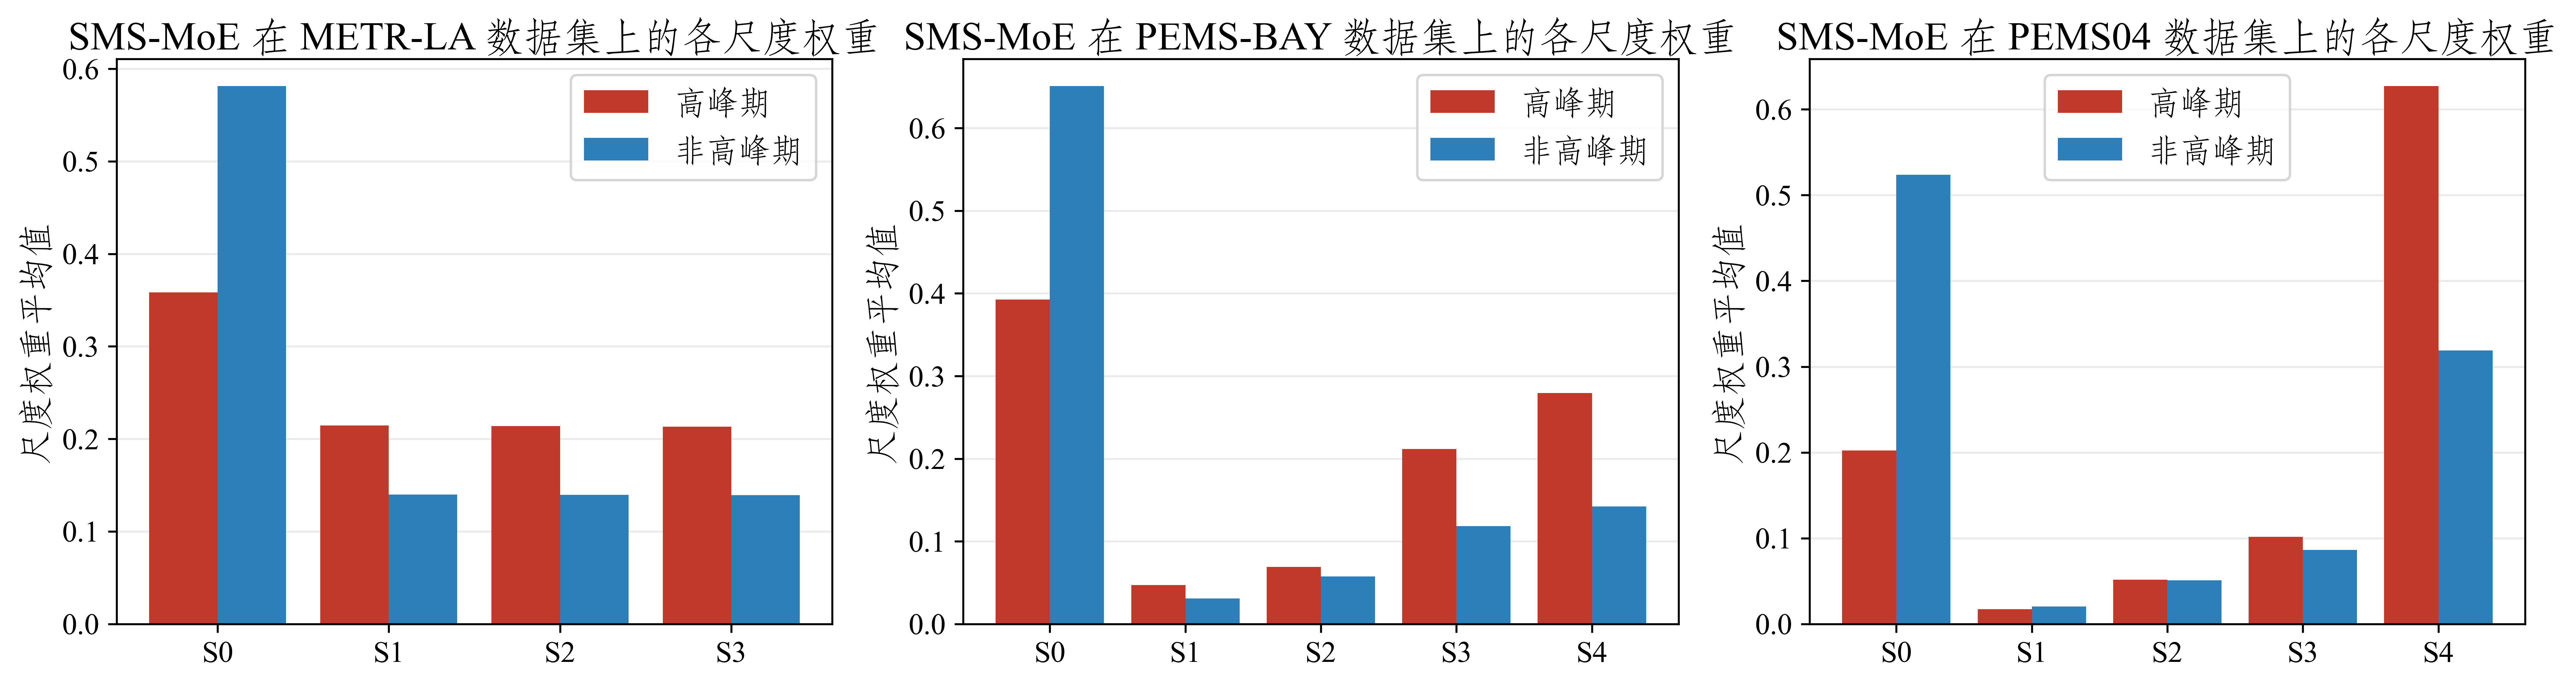
\includegraphics[width=\linewidth]{figure/ch4-scale_gate.png}
    \caption{交通时空预测方法在高峰期与非高峰期时段的尺度权重可视化}
    \label{fig:scale-weight}
\end{figure}

\subsubsection{空间尺度权重的可视化}

为了进一步分析空间多尺度混合专家模块在推理时如何分配尺度权重，本节将训练后的模型，在测试集上高峰期和非高峰期时段的平均尺度权重进行了可视化。本节及后续小节中，将每日 $7{:}00$--$10{:}00$ 和 $16{:}00$--$19{:}00$ 视为高峰期时段，其余时间视为非高峰期时段。

如图~\ref{fig:scale-weight} 所示，在非高峰期时段，三个数据集的原始尺度均持续获得主导权重。这说明当交通状态相对稳定时，空间多尺度混合专家模块主要依赖原始尺度图，因为它保留了更丰富的全局信息。相比之下，在高峰期时段，原始尺度的权重明显下降，不再占据主导地位，而其他尺度的权重上升；在 PEMS-BAY 和 PEMS04 上，这些权重还随尺度增大而增加。这一变化说明，在部分节点交通流量较大的高峰期状态下，模型会将更多权重分配给较大尺度，以突出显著的局部交通模式。上述结果表明，空间多尺度混合专家模块能够根据高峰期和非高峰期交通条件动态重新分配尺度权重，从而学习时间自适应的空间多尺度表示。

\subsubsection{专家路由模式的可视化}

本节在 METR-LA 和 PEMS04 上可视化静动态双混合专家模块在高峰期和非高峰期时段的专家激活模式。具体而言，本节收集推理阶段 SD-MoE 的专家激活统计，并观察路由行为在高峰期和非高峰期条件下的变化。如图~\ref{fig:vis-routing-metr} 和图~\ref{fig:vis-routing-pems04} 所示，在两个数据集上，DyG-MoE 动态图混合专家（左）和 SG-MoE 静态图混合专家（右）的激活频率在高峰期与非高峰期时段均存在明显差异。这种不同的专家路由模式表明，SD-MoE 能够根据时间交通动态自适应选择不同专家，从而在不同交通条件下自适应捕捉时空模式。

\begin{figure}[t!]
    \centering
    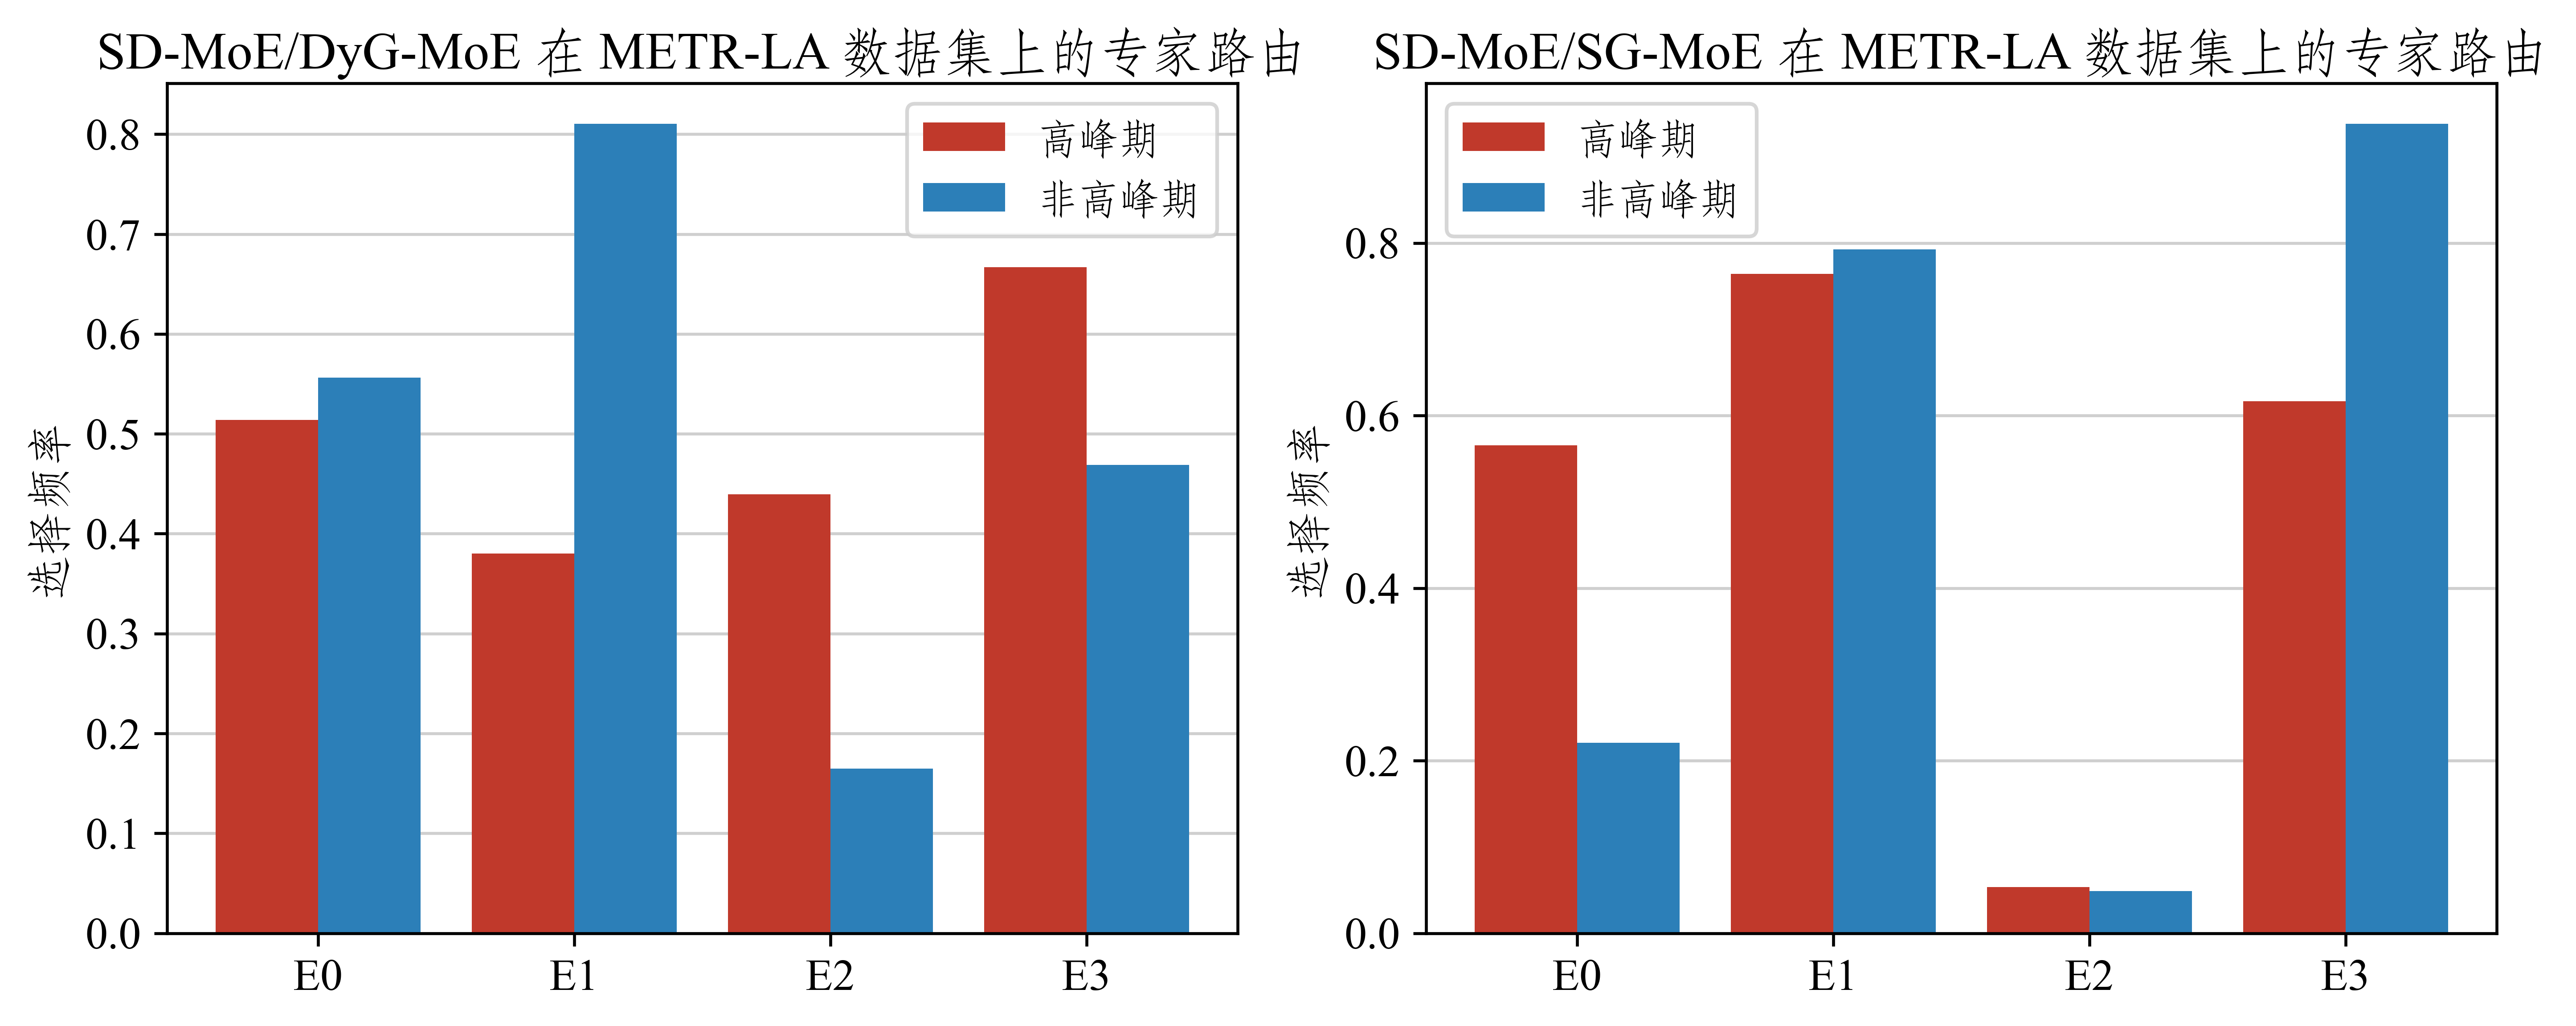
\includegraphics[width=\linewidth]{figure/ch4-METR-LA-routing.png}
\caption{交通时空预测方法在 METR-LA 数据集上的专家路由热力图}
\label{fig:vis-routing-metr}
\end{figure}

\begin{figure}[t!]
    \centering
    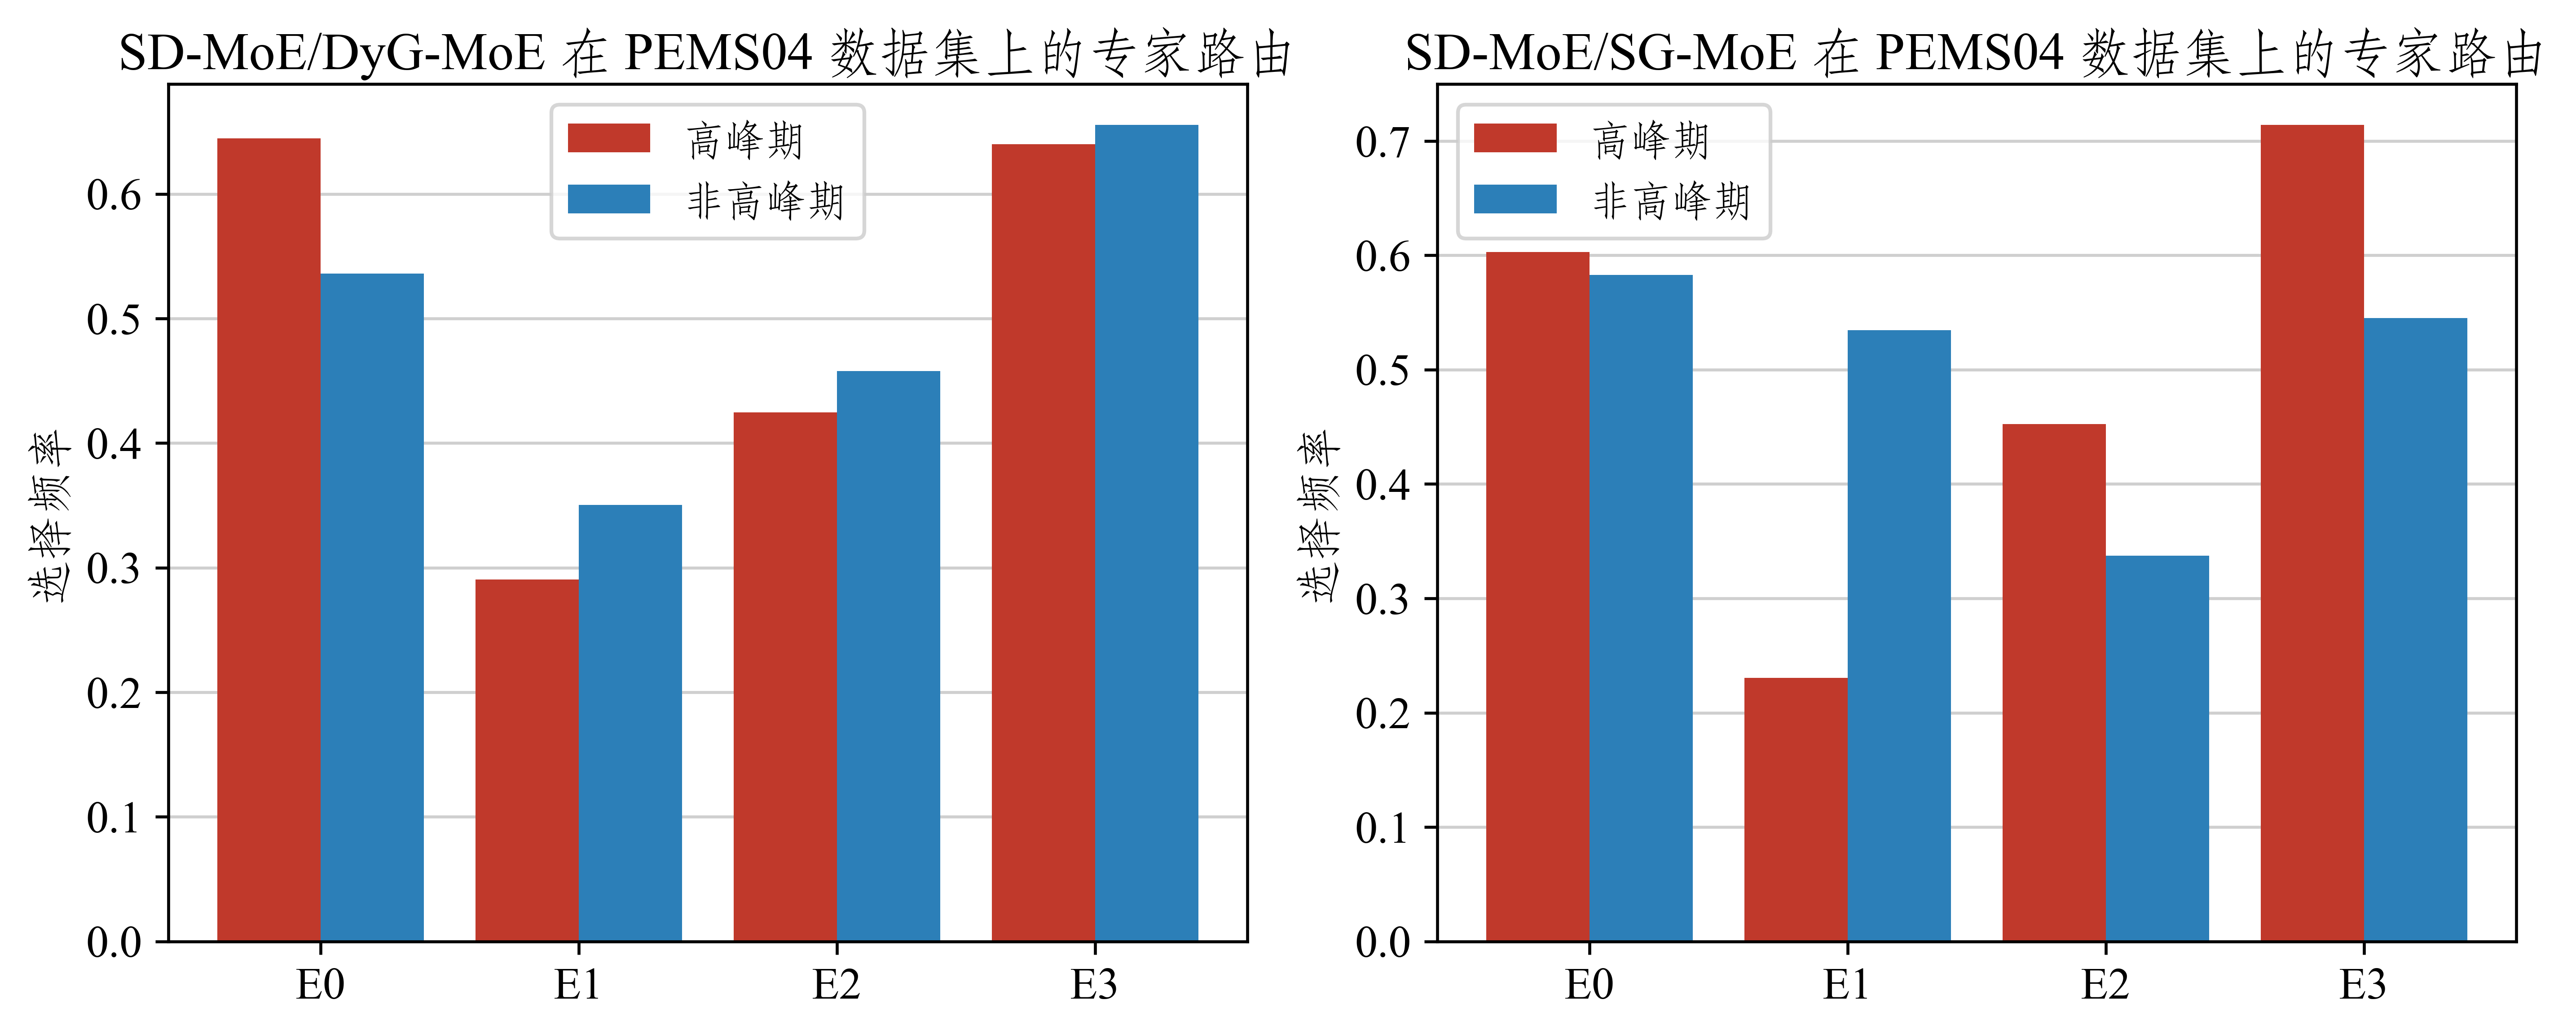
\includegraphics[width=\linewidth]{figure/ch4-PEMS04-routing.png}
    \caption{交通时空预测方法在 PEMS04 数据集上的专家路由热力图}
\label{fig:vis-routing-pems04}
\end{figure}

\begin{figure}[t!]
    \centering
    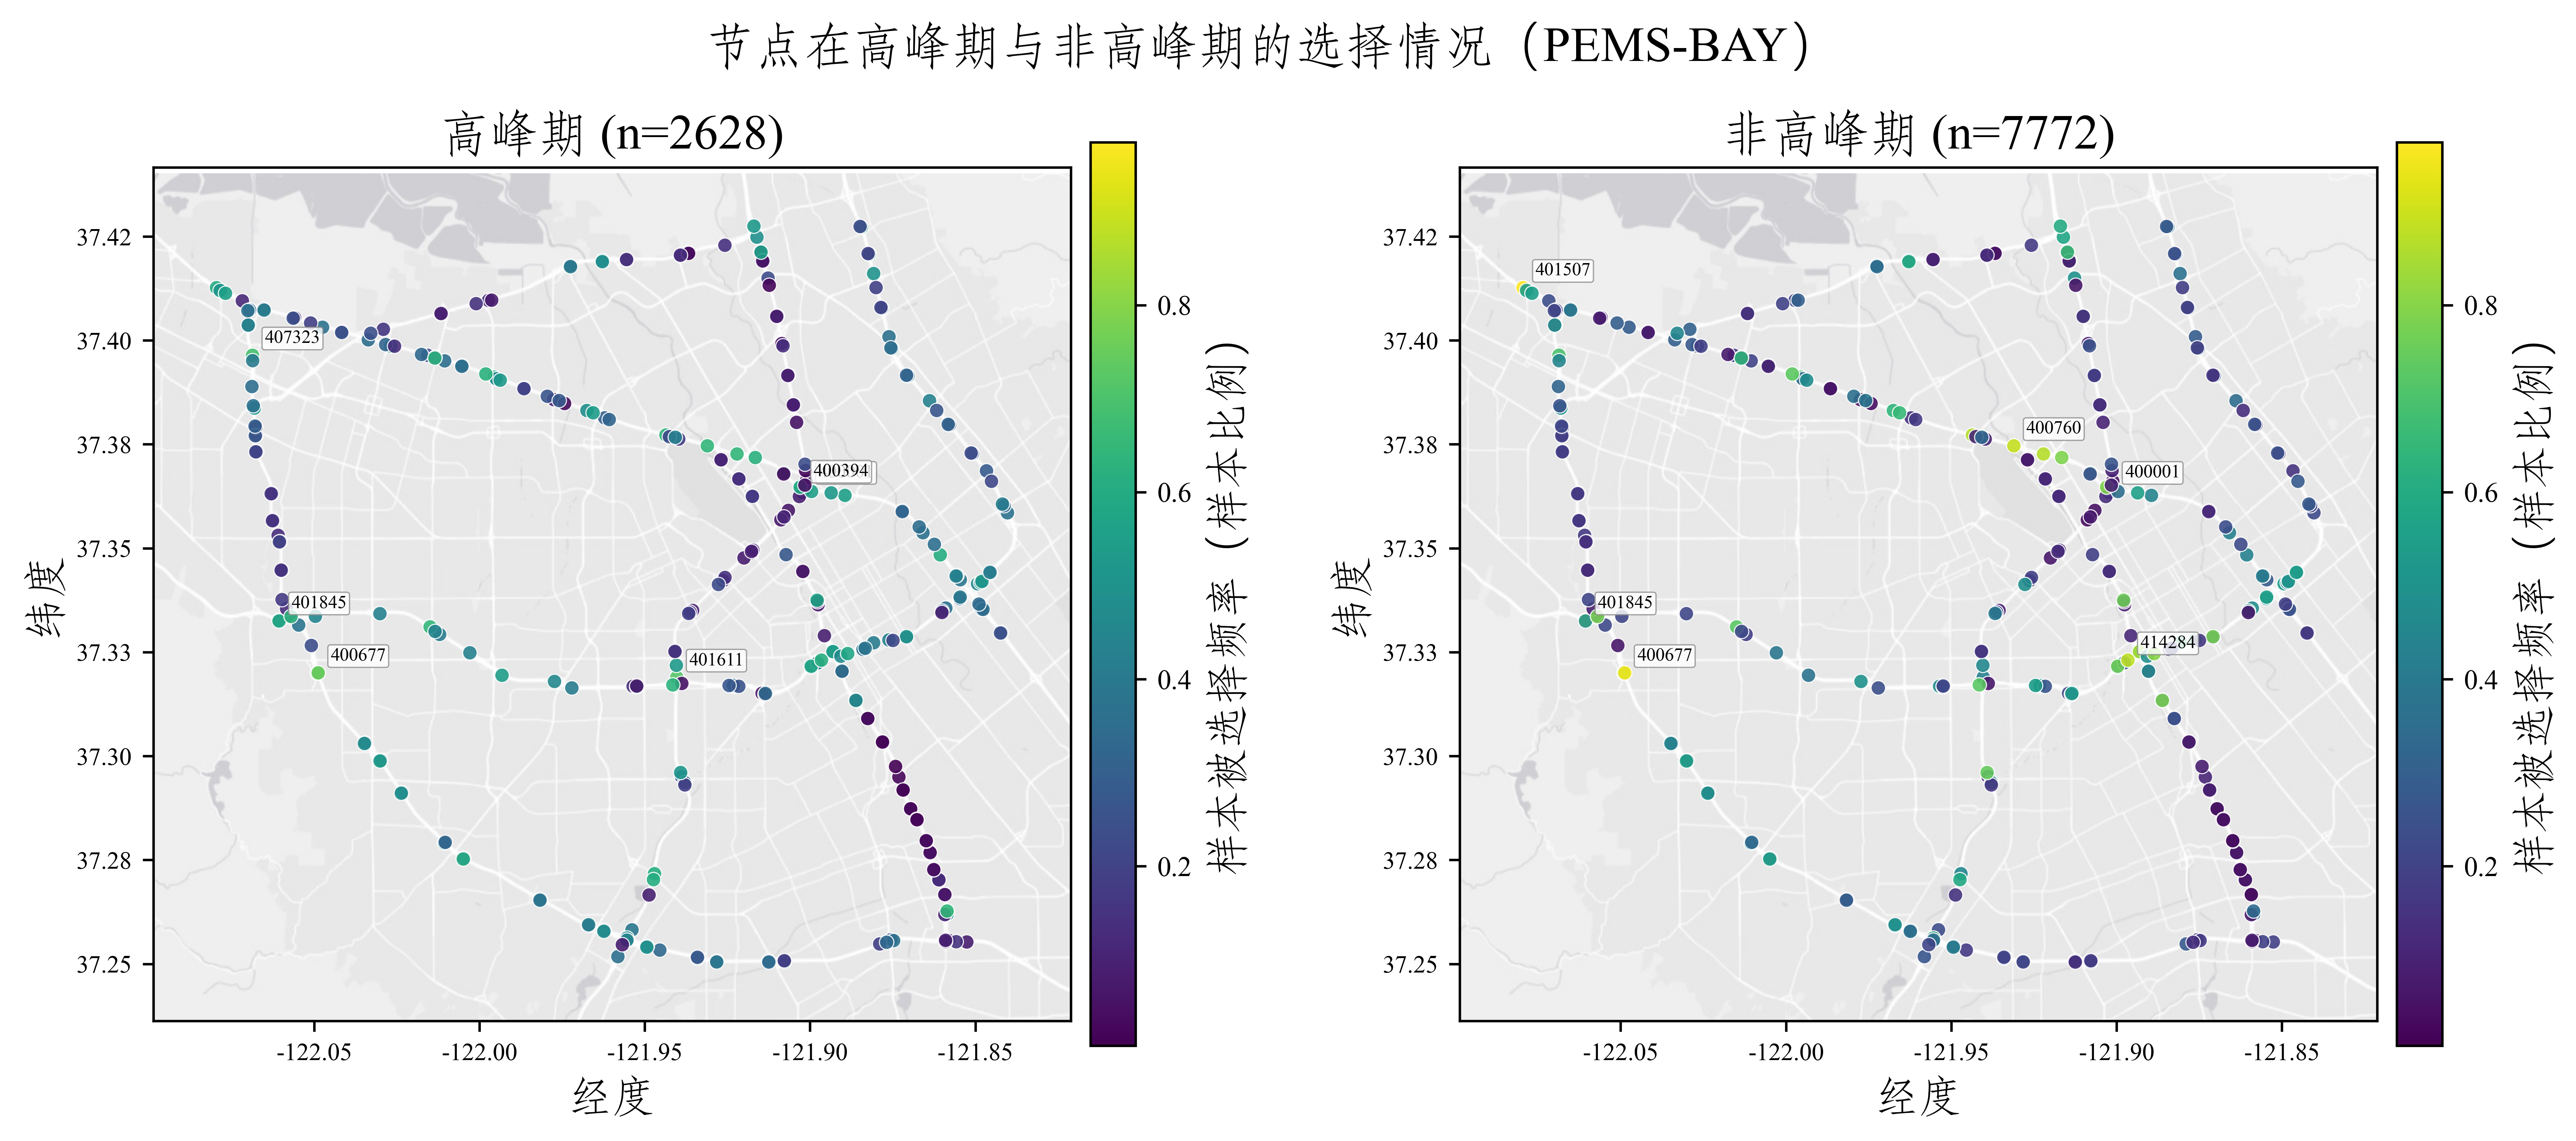
\includegraphics[width=\linewidth]{figure/ch4-nodeselection_PEMS-BAY_peak_vs_offfpeak.png}
    \caption{交通时空预测方法在 PEMS-BAY 数据集上的节点选择频率}
    \label{fig:nodeSelect-twoMaps}
    \end{figure}
    
\begin{figure}[t!]
    \centering
    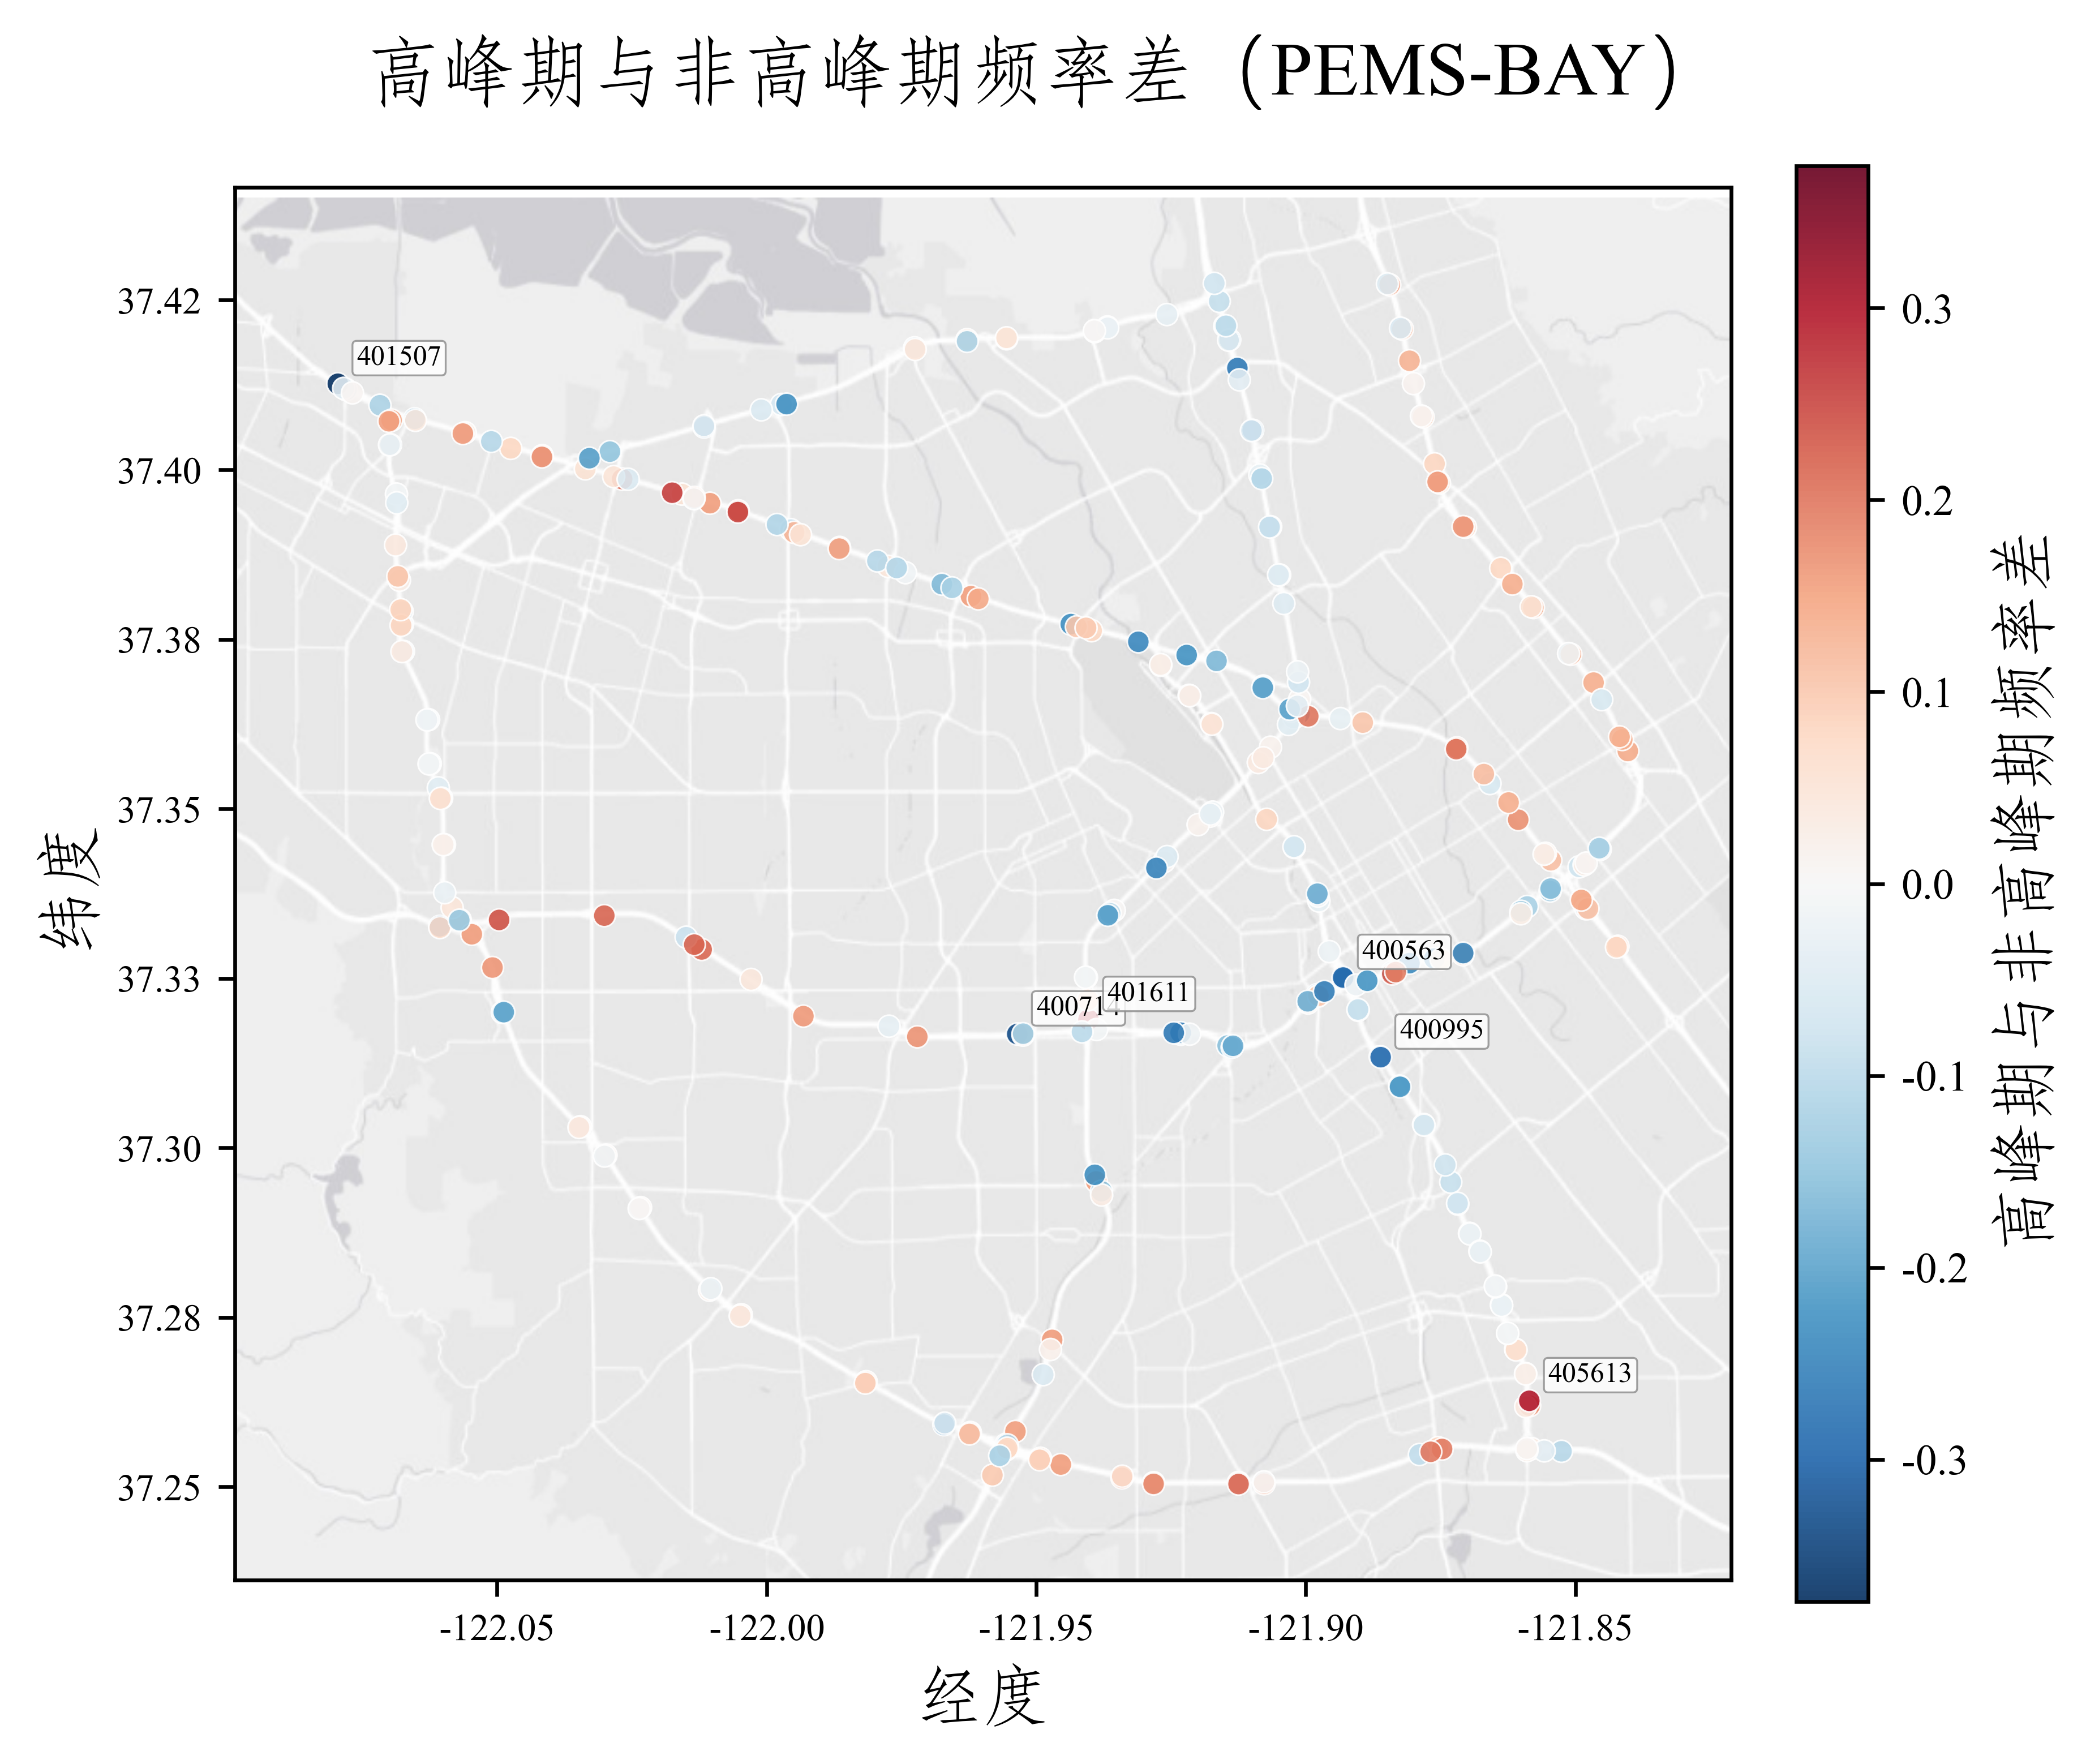
\includegraphics[width=0.49\linewidth]{figure/ch4-nodeselection_PEMS-BAY_diff_map.png}
    \hfill
    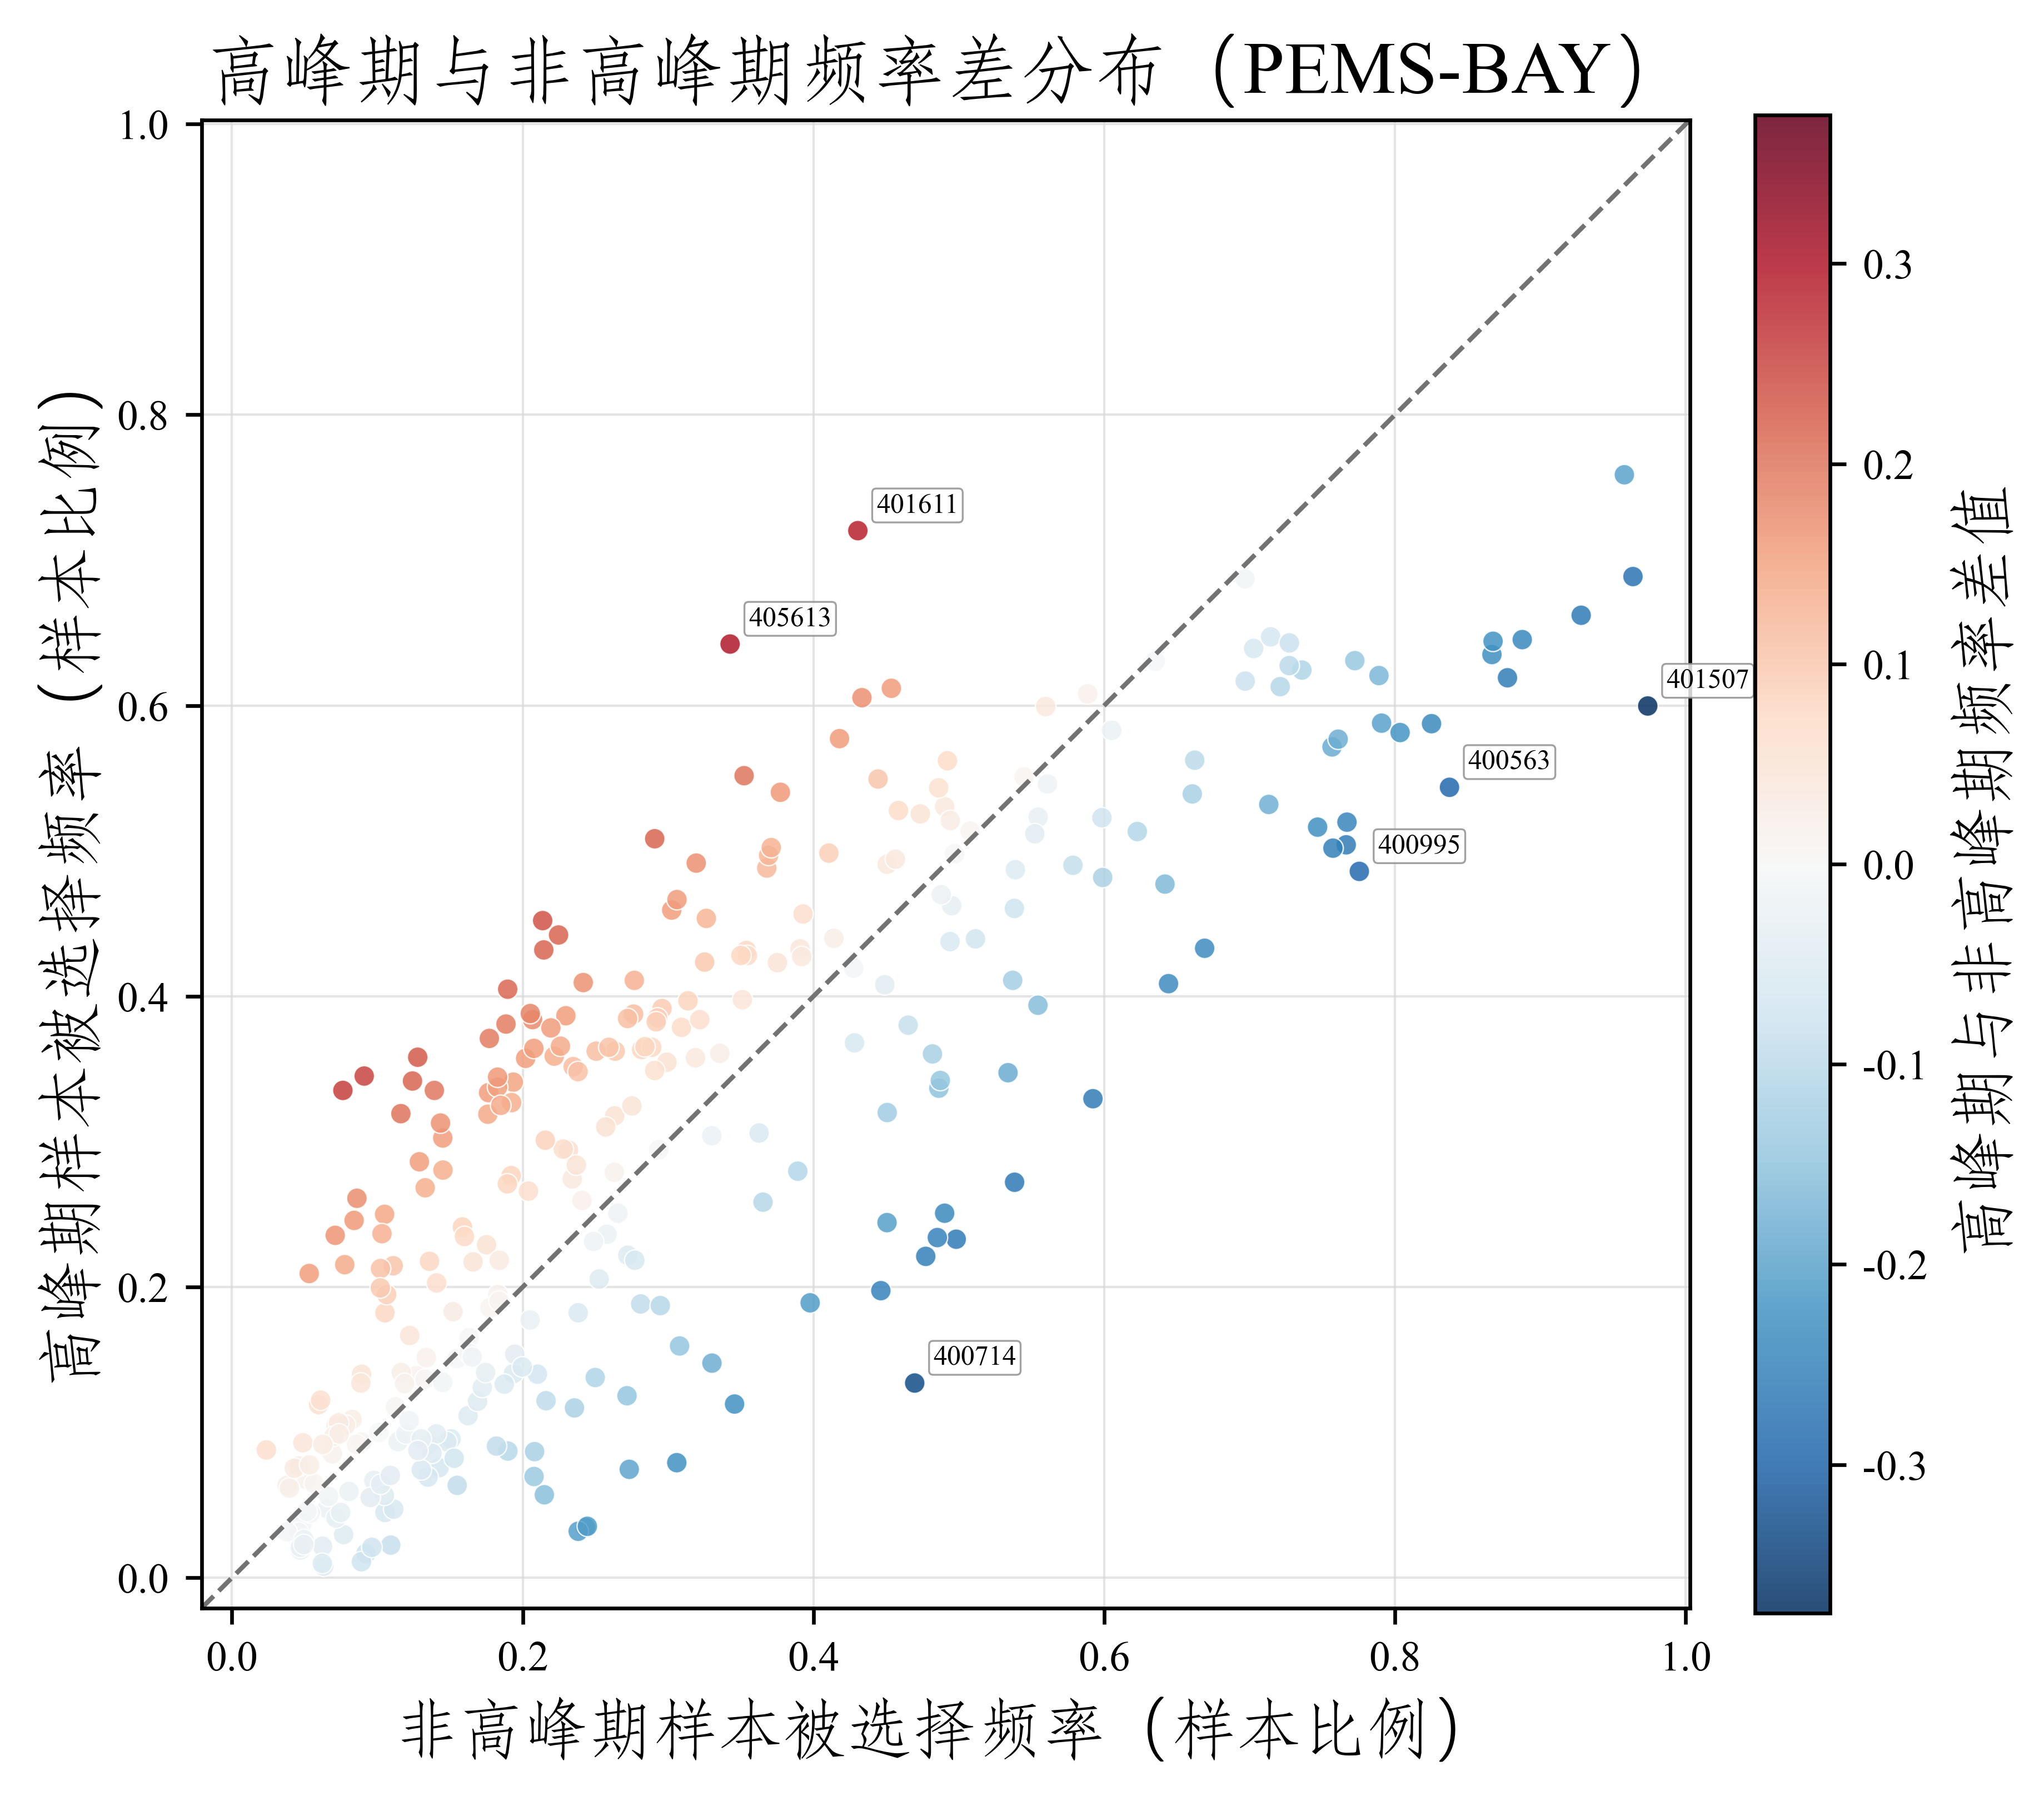
\includegraphics[width=0.49\linewidth]{figure/ch4-nodeselection_PEMS-BAY_scatter.png}
    \caption{交通时空预测方法在 PEMS-BAY 数据集上的节点选择频率差异}
    \label{fig:nodeSelect-diffMap}
\end{figure}

\subsubsection{空间多尺度上下文的可视化}

为了更好地理解学习到的空间尺度，本节收集了在 PEMS-BAY 数据集上，本章方法的空间多尺度混合专家模块在推理时构造子图时的节点选择统计。具体而言，本节在高峰期和非高峰期时段分别统计每个节点被选择的频率，并标注选择频率最高的六个节点编号，如图~\ref{fig:nodeSelect-twoMaps} 所示。

进一步地，本节可视化高峰期与非高峰期节点选择频率之间的差异。如图~\ref{fig:nodeSelect-diffMap} 左侧所示，在高峰期时段，被选择节点主要沿主干道分布，集中在交通流量较大的路段；而在非高峰期时段，被选择节点更倾向集中于主干道交叉口附近。这说明模型在高峰期更关注路段级交通动态，而在非高峰期则转向对区域级整体交通条件的表示。

图~\ref{fig:nodeSelect-diffMap} 右侧子图为高峰期减非高峰期节点频率差异的散点图。散点图的横纵坐标分别比较了归一化后的高峰期和非高峰期节点选择频率。对角线将高峰期减非高峰期选择频率的正差区域与负差区域分开：左上侧为正差，右下侧为负差。大多数点位于右下区域，说明高峰期选择集中在少数高流量路段，而非高峰期选择分布在更广泛的区域级节点上。该结果进一步说明空间多尺度混合专家模块能够根据交通状态改变节点选择范围，从而形成具有时间自适应性的空间多尺度表示。


\section{本章小结}

本章针对具有显式空间图结构的交通预测问题，提出了一种融合自适应空间多尺度建模与静动态双混合专家的预测框架。与现有方法依赖距离、聚类或节点相似性等先验知识构造固定空间尺度的做法不同，本章通过图池化以数据驱动方式逐步构造多个空间尺度，并利用尺度专家和尺度自适应融合提取尺度特异性特征。该设计使模型能够根据当前交通状态动态调整不同尺度的贡献，从而同时捕捉局部路段拥堵传播和区域级宏观交通模式。

在空间建模方面，本章通过图卷积和可学习骨干节点构造尺度专家，并利用散布对齐、输入自适应尺度门控和自顶向下混合实现多尺度空间特征融合。该过程不依赖固定图划分，能够根据输入节点重要性动态选择保留节点，从而保留原始图细节和粗尺度宏观结构。理论复杂度分析表明，稀疏专家激活和图池化有助于控制大规模图上的计算开销。

在时空依赖建模方面，本章使用静态图混合专家和动态图混合专家分别处理显式道路拓扑和隐式时空交互。静态图专家通过图卷积保留由路网连接决定的结构先验；动态图专家通过节点级全注意力建模不受局部邻域限制且随时间变化的跨节点依赖。两个模块均采用稀疏激活和噪声门控路由，能够在不显著增加计算开销的情况下提高模型容量，并通过门控融合自适应整合空间多尺度特征和静动态时空特征。

在 6 个公开交通数据集上的实验表明，本章方法在多数预测步和平均指标上取得较优或接近最优的结果。消融实验验证了空间多尺度混合专家、静态图专家、动态图专家、负载均衡损失和骨干节点的作用；尺度因子、专家数量和 Top-$k$ 分析进一步说明了尺度自适应、稀疏激活和路由参数对预测性能的影响。长时预测和资源开销实验表明，模型在较长预测范围内仍保持较稳定表现，同时借助稀疏激活控制了显存占用。可视化结果也表明，模型在高峰期和非高峰期时段会选择不同的空间尺度和专家，能够学习时间自适应的空间多尺度表示。

综上，本章将第3章中的多尺度建模与混合专家思想从时间维度扩展到空间图结构，并进一步联合建模静态与动态时空依赖。与第3章共同构成了一套从一般多元时间序列预测到结构化时空交通预测的递进研究框架，分别验证了时空多尺度建模和混合专家系统在时间域与空间域中的有效性。
